\chapter{Downwash Estimation}
\label{ch:workobject}
\markboth{Downwash Estimation}{}

\begin{flushright}
	{\smaller
		\textit{The important thing is not to stop questioning.\\  Curiosity has its own reason for existing.}\\
		-- Albert Einstein}
\end{flushright}

In order to evaluate the characteristics of longitudinal stability of an aircraft it's necessary to assess the flow direction aft of the wing. The contribution of horizontal tail surface to the airplane equilibrium and stability, in fact, strongly depends on the flow direction. The purpose of this chapter is to introduce and evaluate the downwash gradient due from the wing's vortex system, considering a dependence of the downwash angle from the absolute angle of attack. 

\section{Theoretical background}

Due to the finite extension of the wing the lift distribution in span is not uniform. For this reason the difference of pressure between upper and lower surfaces generates a movement of air around the wingtips. The tendency is for particles of air to move from the region of high pressure around the wing tip to the region of low pressure (for positive lift from the lower wing surface to the upper surface). This made the wing's vortex system that consists of the bound vortex, located at the wing quarter chord and a vortex sheet which rolling up, at the wing tip, in two trailing vortex.\cite{PerkinsHage} \cite{Jacobs:NACA:Rep:648} \\ 

% traduci

\begin{figure}[H]
\centering
{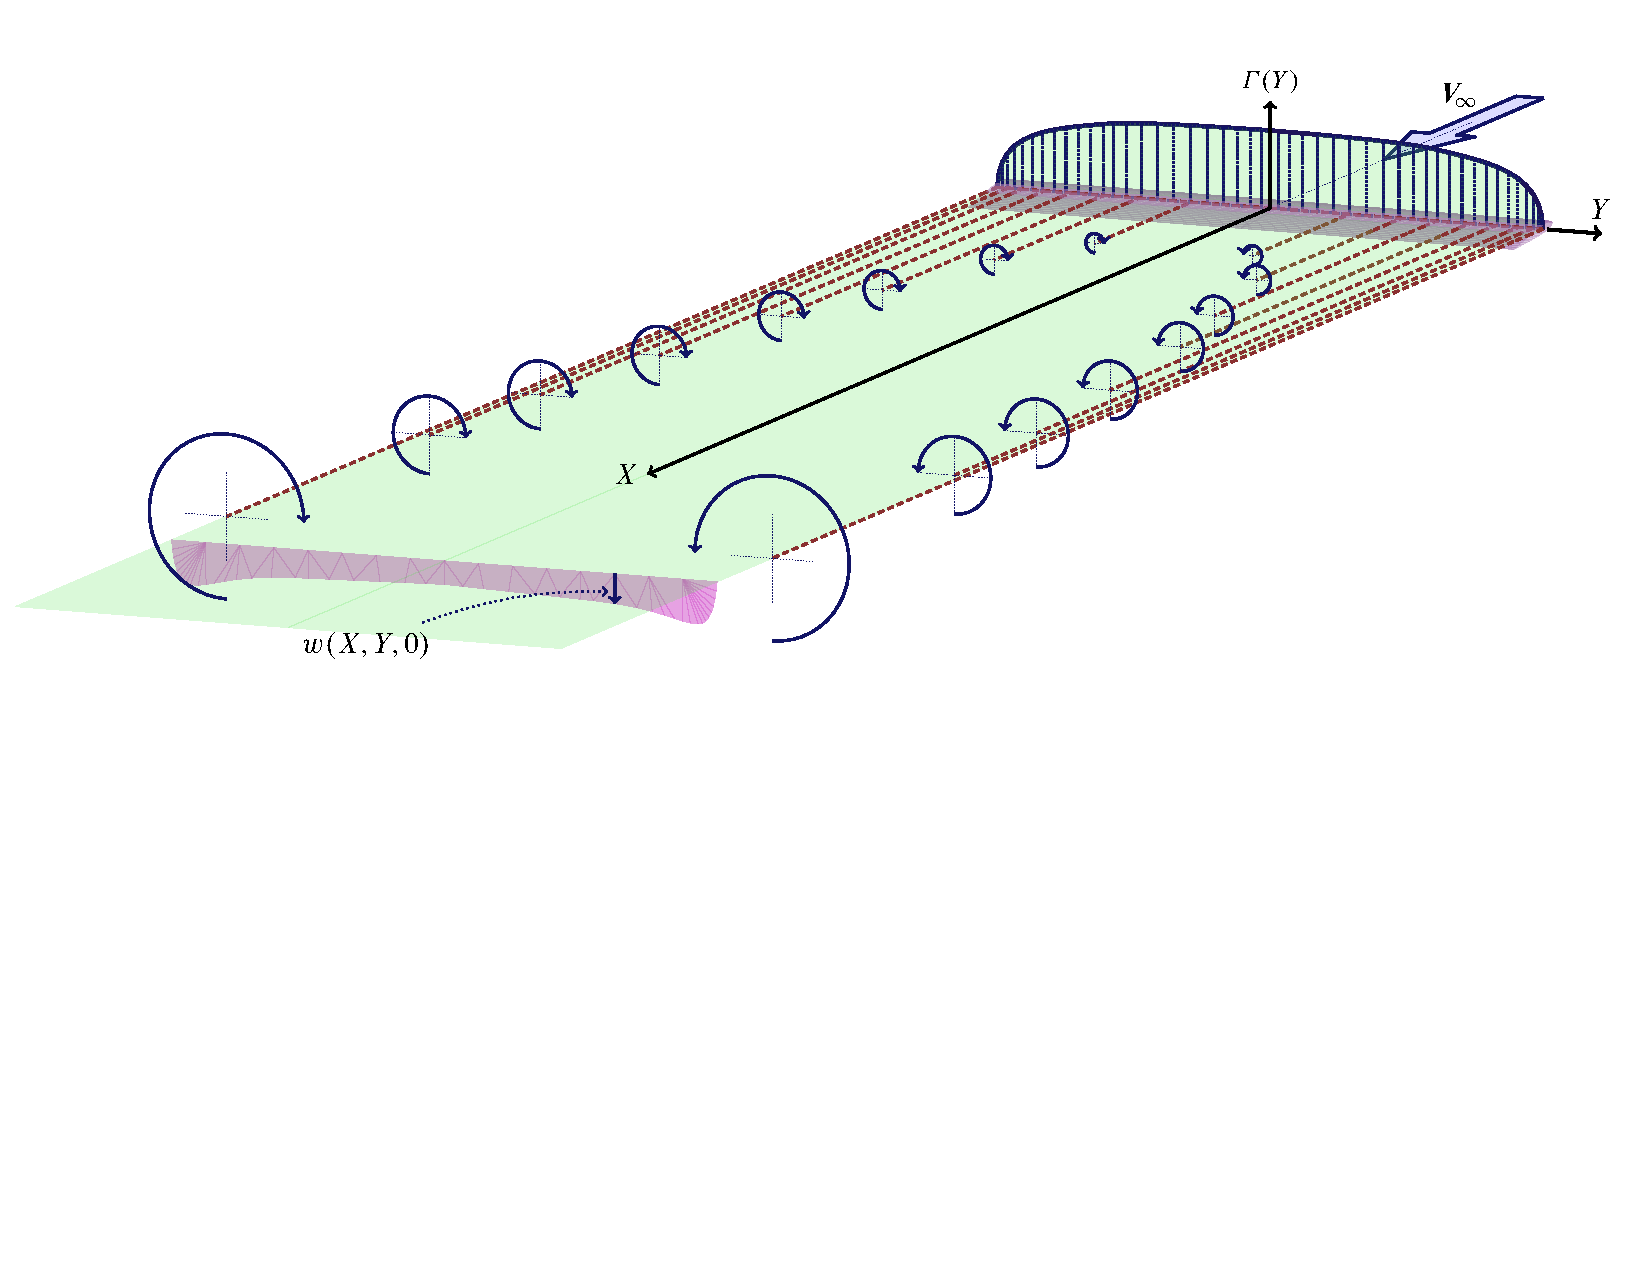
\includegraphics[height=5.7cm]{Immagini/wing_vortex_sheet3.pdf}} 
\caption{The wing vortex sheet.}
\end{figure}

The main effect of this vortex system is to deflect the airflow behind the wing downward relative to the direction of freestream flow. This angle of deviation is known as {\itshape Downwash Angle} $\epsilon$. This phenomenon occurs for every lifting surface, but in subsonic flow a lifting surface also affects the flow forward of itself. In this region the vortex creates an {itshape upwash}, that is an upward flow deflection.\\


\begin{figure}[H]
\centering
{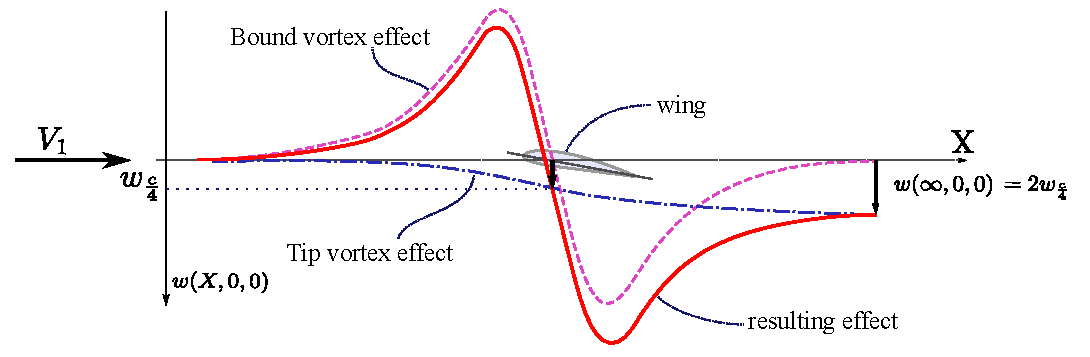
\includegraphics[height=5.16cm]{Immagini/wing_upwash_downwash.pdf}} 
\caption{Upwash and Downwash in a finite wing.}
\end{figure}

As consequence of the downwash behind the wing, the local angle of attack on the horizontal tail is reduced by  $\epsilon$. In order to evaluate the flow direction behind the wing, an other important parameter is the change in downwash angle with angle of attack, that is the {\itshape Downwash Gradient } $\frac{d\epsilon}{d\alpha}$.\\
This parameter depends principally on the location of the horizontal tail respect to the wing and the vortex plane. As first approximation this value could be considered constant in alpha, but more accurately it's possible to evaluate this dependence considering the reference variable for the calculation of the distances. 
If the vertical distance is considered constant, starting from the downwash gradient, the downwash angle is :

\begin{equation}
\epsilon = \frac {d \epsilon}{d \alpha_w} (\alpha_w - \alpha_{0_w})
\end{equation}

\noindent \\ \\
In order to evaluate the downwash gradient we refer to fig. \ref{PerkinsDownwash}, where ``$r \frac{b}{2}$''  is the distance between the aerodynamic center of wing and the aerodynamic center of the horizontal tail. In order to have a greater accuracy it is possible to measure this distance along the diretion of local flow and, consequently, consider it as variable with the angle of attack. The parameter ``$m\frac{b}{2}$' , properly, is the distance between the horizontal tail and the vortex shed plane, but it is possible to approximate it with the distance between the horizontal tail and the wing root chord.\cite{schimidth}

Referring to \cite{Slinger} the equation used in order to evaluate the downwash gradient is the following: 

\begin{equation}
\begin{split}
 \frac{d\epsilon}{d\alpha} &= \frac{K_{\epsilon \Lambda}}{K_{\epsilon _{\Lambda=0}}}  \Biggr ( \frac{r}{r^2+m_{tv}^2} 
 \frac{0.4876}{\sqrt{r^2 + 0.6319 + m_{tv}^2}}  +\\
& \left [1+{ \left( \frac{r^2}{r^2 + 0.7915 + 5.0734 m_{tv}^2} \right) }^{0.3113}  \right ]    \left \{ 1- \sqrt{\frac{m_{tv}^2}{1+m_{tv}^2}} \right \}      \Biggl )    \frac{C_{L_{{\alpha}_w}}}{\pi \AR}
\end{split}
\label{eqPerkinsDownwash}
\end{equation}

\noindent \\
Considering a variable downwash gradient the changing parameters are``$r \frac{b}{2}$'' , $m \frac{b}{2}$ and the slope of the CL vs $\alpha$ curve.

\begin{figure}[H]
\centering
{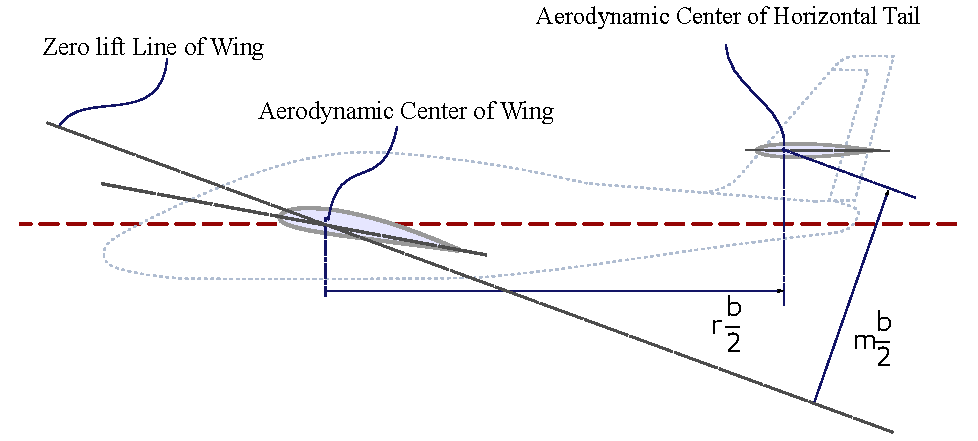
\includegraphics[height=7.3cm]{Immagini/wing_htail_Roskam_eng.pdf}} 
\caption{Dimensions for determination of Downwash Gradient, considering constant distances.}
\label{PerkinsDownwash}
\end{figure} 

The two $K_{\epsilon}$ terms in the eq~\ref{eqPerkinsDownwash} accounting for the wing sweep angle effect are defined as follow ( where $\Lambda $ expressed in radians):

\begin{equation}
K_{\epsilon \Lambda} = \frac{ 0.1124 + 0.1265 \Lambda + 0.1766 \Lambda^2}{r^2} + \frac{0.1024}{r} +2
\end{equation}

\begin{equation}
K_{\epsilon _{\Lambda=0}} = \frac{ 0.1124 }{r^2} + \frac{0.1024}{r} +2
\end{equation}

These two terms are constant with $\alpha$ because  it does not appear the variable parameter in them.


\section{Java Class Architecture}

In order to simplify the calculation of downwash, as mentioned, it is possible to assume the downwash gradient constant with the angle of attack. In this case the reference line to calculate the distance along z axis is the plane from the wing root chord or else the zero-lift line of the wing.\\
To obtain a more accurate analysis it is possible to consider the variation in alpha of the downwash gradient. So the reference line of wing it is not costant, but is the vortex sheed plane. The location of this plane depends from the value of downwash, but this location is itself necessary to evaluate the downwash. So it is necessary an iterative process in which the position of the vortex reference line at alpha is calculated from the value of downwash gradient at previous step.\\ 

In this process the reference angle of attack is the absolute angle $\alpha_a$, that is the angle between the flow direction and the zero lift line of the wing. This choice is necessary because for $\alpha_a = 0$ it is possible to assume the downwash zero, but the downwash gradient is not null. In this way it is possible to assume the downwash value in the first step of the iteration and to continue for each step with the previous value as first attempt.
In view of stability, however, the reference angle of attack is the $\alpha_B$. There two angles they are related by the relation: $ \alpha_B =\alpha_{0L} - i_w + \alpha_a $. \\The relation between the angles is in the fig \ref{anglesDef}.

\begin{figure}[H]
\centering
{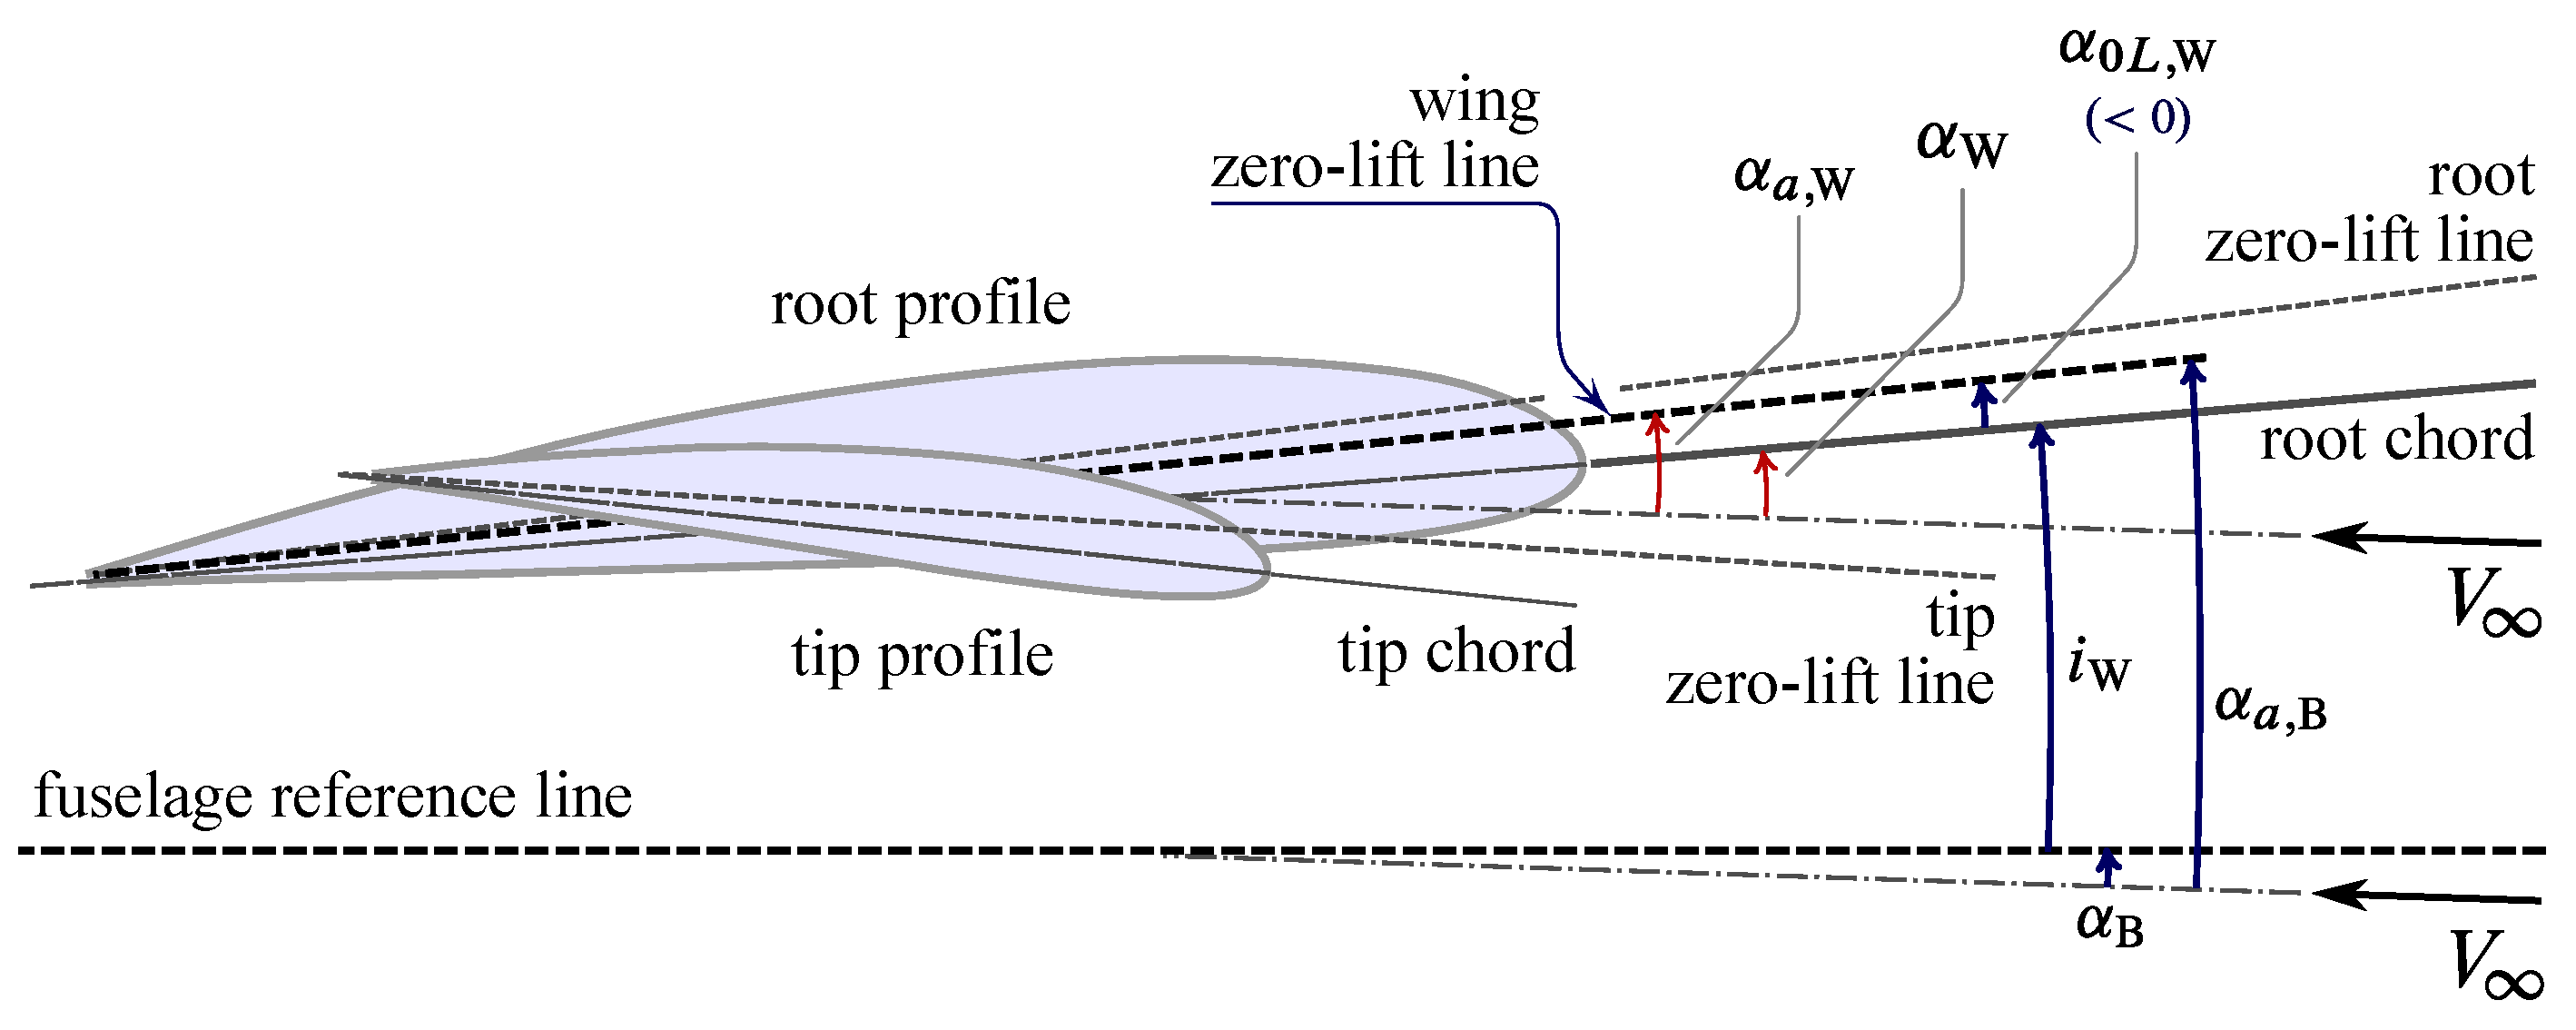
\includegraphics[height=6cm]{Immagini/Wing_Alpha_Zero_List.pdf}} 
\caption{Definition of wing angles.}
\label{anglesDef}
\end{figure} 


The downwash angle is calculated by a class named \texttt{DownwashCalculator}. The builder of this class defines and assigns all the geometrical variables, necessary to implement the calculation and defines an array of $C_{L_{\alpha}}$. The  \texttt{DownwashCalculator} class has seven methods and some overloads. The methods are explained in the table~\ref{table:Table1}. The methods will be explained more in detail below.

\begin{table}[H]
\begin{tabular}{p{7cm}p{7.5cm}}
\toprule
 \\[0.1	cm] 
\lstinline[language=Java]!calculateDownwashGradientConstantDelft! & This method calculates the downwash gradient  considering the vertical distance geometrical and constant\\ \hline \\[0.1	cm] 
\lstinline[language=Java]!calculateDownwashNonLinearDelft! &This method calculates the downwash considering a non constant downwash gradient.  \\ \hline \\ [0.1cm]
\lstinline[language=Java]!getDownwashAtAlphaBody! & This method returns the value of downwash angle, interpolating data filled before.\\ \hline \\[0.1cm]
\lstinline[language=Java]!calculateZDistanceZeroLift!	& This method calculates the distance between the aerodynamic centre of horizontal tail and the zero lift line of the wing. \\ \hline \\[0.1cm]
\lstinline[language=Java]!Plot Methods ...! & Using these methods it is possible to plot the downwash angle, the downwash gradient and the distance in function of $\alpha_{B}$ \\
\bottomrule
\end{tabular}
\caption{Methods of \texttt{DownwashCalculator} class.}
\label{table:Table1}
\end{table}


\subsection{Constant Downwash Gradient}
In order to evaluate the downwash angle case of constant downwash gradient it is necessary only to call the method \texttt{calculateDownwashGradientConstantDelft} using the distance from aerodynamic center of horizontal tail and the alpha zero lift line as input. It is possible to calculate this distance geometrically using the method \texttt{calculateZ DistanceZeroLift} of the same class. The choice to calculate separately the distance and the downwash gradient is made to reuse the method to calculate downwash gradient simply varying the input distance. \\ 
This method has the downwash gradient as output. To obtain the angle of downwash it simply need to multiply the output value and the absolute angle of attack. 

\begin{figure}[H]
\centering
{\includegraphics[height=8cm, angle=90]{Immagini/linearDownwash_2.pdf}} 
\caption{Flow chart of the calculation of linear downwash angle.}
\label{flowchartangles}
\end{figure} 



\subsection{Variable Downwash Gradient}

In order to evaluate the non-constant downwash gradient it is necessary to use the method \texttt{calculateDownwashNonLinearDelft}. 
This method calculates the downwash gradient using Slingerland formula. The downwash gradient is considered variable with alpha absolute. 
\\ \\
The distances  considered in the formula are variable and they are measured from the vortex shed plane. These distances have been calculated referring to the geometrical construction proposed  by \cite{uninagiordano}.\\
First of all it is necessary to evaluate the geometrical distances $m_0$ and $x_0$, then it is possible to evaluate step-by-step the other distances which, fixed geometry, only depend with alpha.\\ Starting from a value of  $\alpha_a = 0^{\circ}$ and proceeding with an increase of angle of attack equal to $ \upDelta \alpha$, the distances are the following ( see fig. \ref{armdefinitiondownwa}).

\begin{itemize}
\item {\bfseries $x_0$}  $\rightarrow$ distance between the aerodynamic center of the wing and the aerodynamic center of the horizontal tail calculated along the x axis.  
\item {\bfseries $m_0$}  $\rightarrow$ distance between the aerodynamic center of the horizontal tail and the horizontal line passing through the trailing edge of the airfoil root of the wing.
\item {\bfseries d}  $\rightarrow$ distance between the trailing edge of the wing and the aerodynamic center of the horizontal tail. Considering the triangle $ \hat{BCD} $ it is possible evaluate the hypotenuse as follows:
\begin{equation}
d= \sqrt{CD^2 + BD^2}
\end{equation} 
where CD is the distance $m_0$ defined before and it is possible to evaluate the distance BD geometrically:
\begin{equation}
BD = x_0 - \frac{3}{4} c_r \cos(i_w)
\end{equation}
\item {\bfseries $\psi$}  $\rightarrow$ This is the angle between the distance d and the horizontal reference line.
\begin{equation}
\psi = \arctan(\frac{m_0}{BD})
\end{equation}
\end{itemize}

Starting from these geometrical values it is possible to evaluate the distances m and r for each angle of attack.

\begin{itemize}
	\item $m|_i = d \sin(\psi + i_w - \alpha_{0_L}- i \upDelta \alpha + \epsilon)$
	\item $x|_i =  d \cos(\psi + i_w - \alpha_{0_L}- i \upDelta \alpha + \epsilon) + \frac{3}{4} c_r \cos(-\alpha_{0_L} - i \upDelta \alpha+ + \epsilon)$
\end{itemize}

\begin{figure}[H]
\centering
{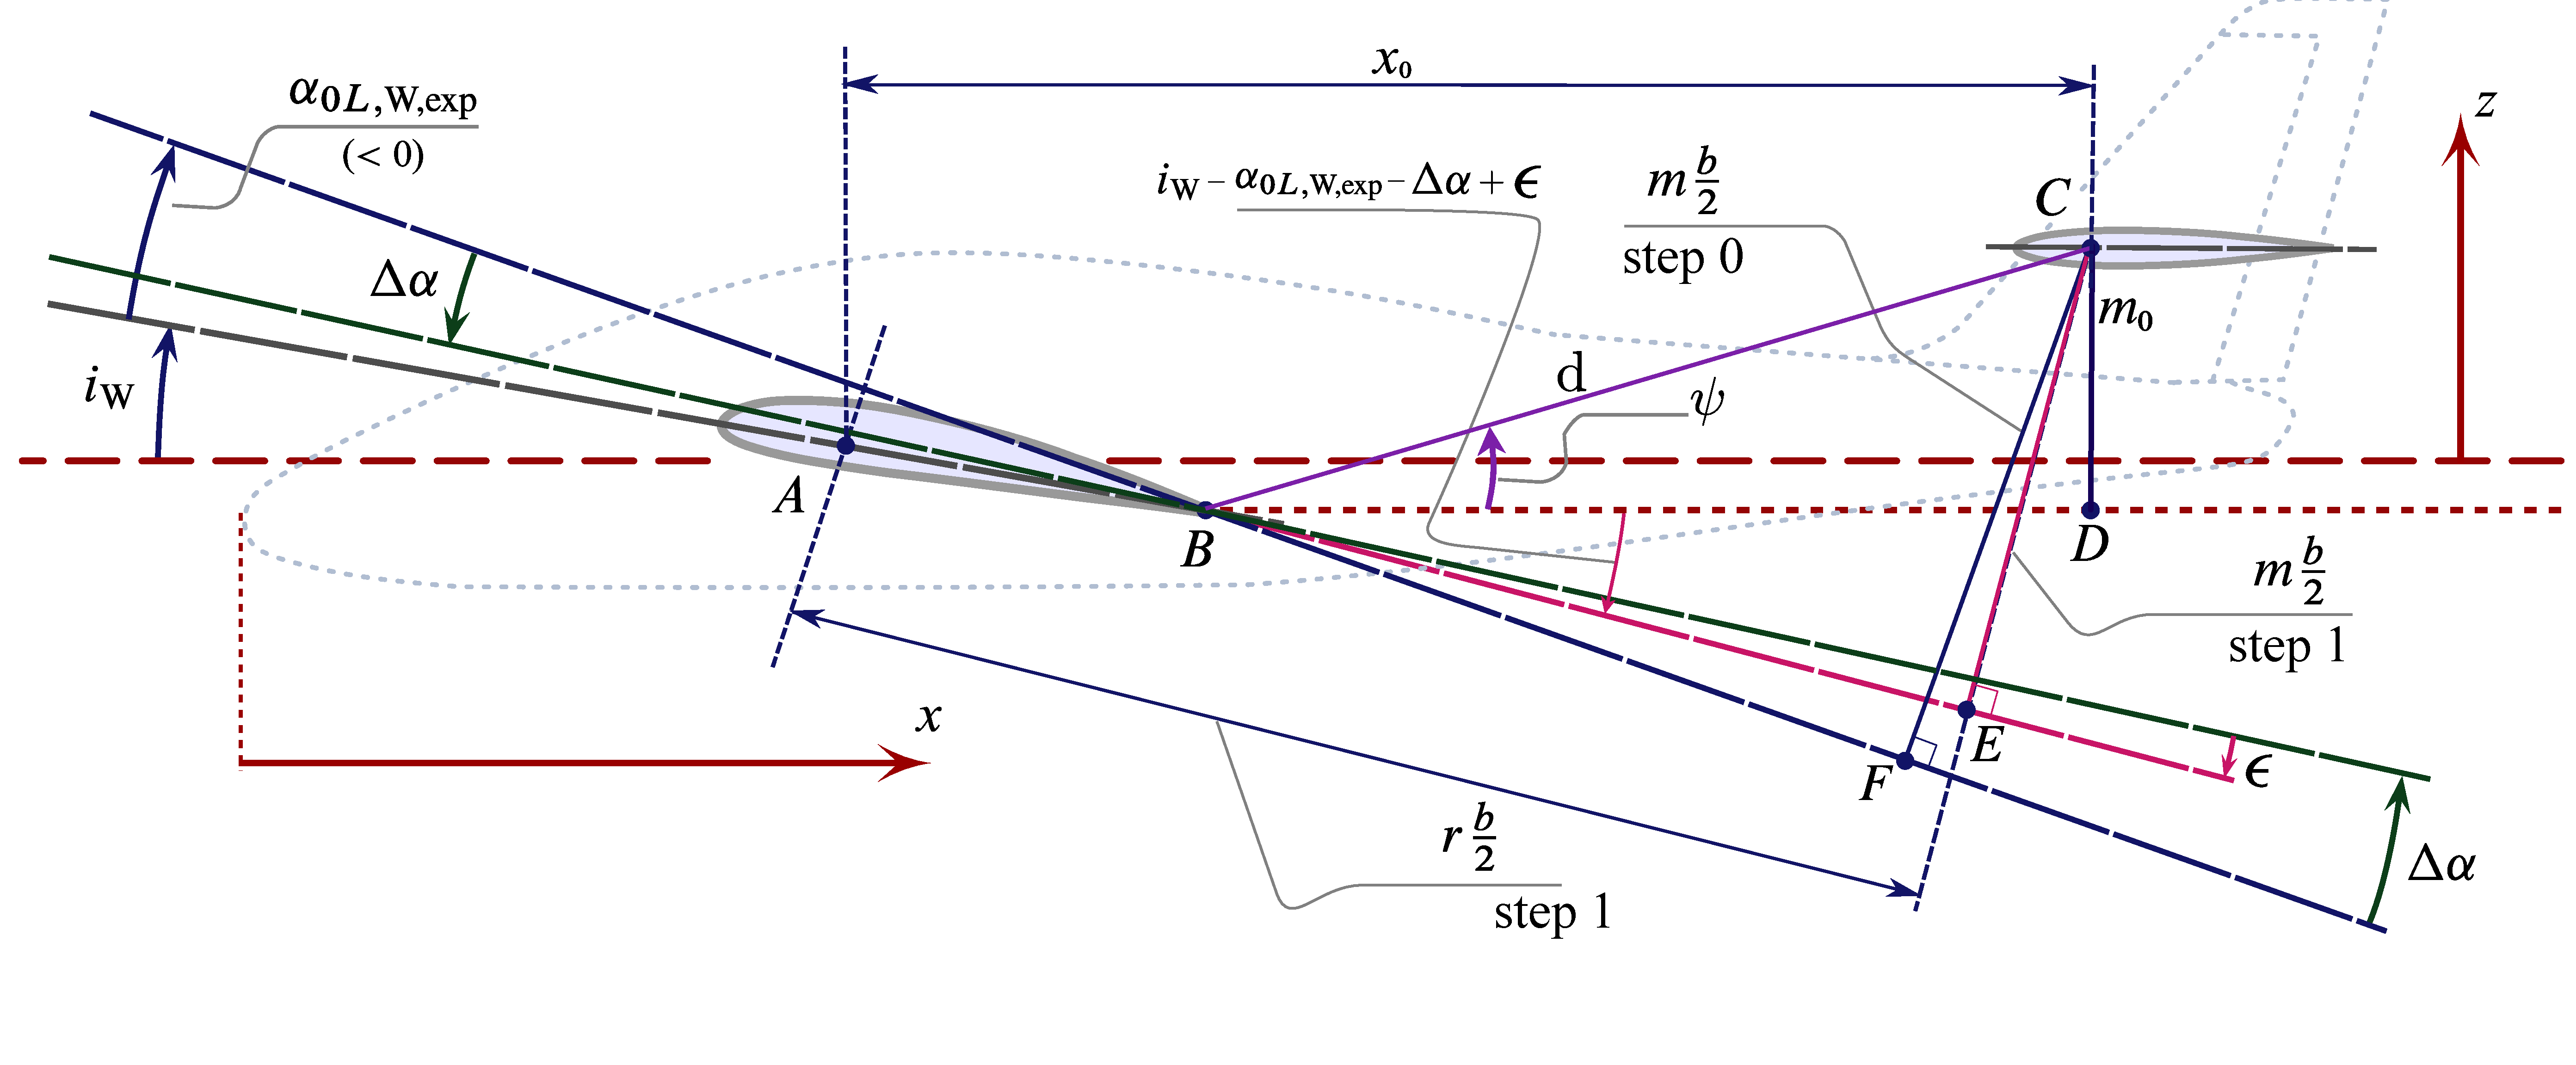
\includegraphics[height=6.69cm]{Immagini/arms_definitions_mod.pdf}} 
\caption{Arm definitions for downwash gradient evaluation.}
\label{armdefinitiondownwa}
\end{figure} 


The \texttt{calculateDownwashNonLinearDelft} method works uses these distances and through the following steps:

\begin{enumerate}

\item First of all this method creates an array of absolute angle of attack starting from $\alpha = 0^{\circ}$ to  $\alpha = 20^{\circ}$ with a step of $0.25^{\circ}$.
\item The results array are initialized ( $\alpha_a$ , $\alpha_B$ , $\frac{d\epsilon}{d\alpha}$ ,  $\epsilon$ , $m  \frac{b}{2}$ ). 
\item For the first step the state is the following:

\begin{itemize}
\item $\alpha_a = 0^{\circ}$ 
\item $\alpha_B =\alpha_{0L} - i_w$ 
\item $\frac{d\epsilon}{d\alpha}$  is the constant value 
\item  $m  = d \sin(\phi + i_w -\alpha_{0_L})$ 
\item  $r  = d \cos(\phi + i_w -\alpha_{0_L}) + 0.75 c_r \cos(-\alpha_{0_L}) $ 
\item $\epsilon = 0$ 
\end{itemize}

\item Starting from the second step the process is iterative. Starting from $\alpha_a = 0^{\circ}$ the absolute angle of attack increase of $\upDelta \alpha$. For the step i:

%\begin{enumerate}
%\item $\alpha_a = i \Delta \alpha$ 
%\item $\epsilon_{temp}= \frac{d\epsilon}{d\alpha} \right |_{i-1} *  \alpha_a $%\right |_{i}$ 
%\item  $m  \frac{b}{2} _{temp} $ is calculated considering the temporary value of downwash angle.
%\item $\frac{d\epsilon}{d\alpha}_{temp}$ is calculated using the formula and the temporary value of distance.
%\item $\epsilon_{i}=  \frac{d\epsilon}{d\alpha}\right_{temp} *  \alpha_a \right |_{i}$ 
%\item  $m  \frac{b}{2} _{i} $ is calculated considering the new value of downwash angle.
%\item $\frac{d\epsilon}{d\alpha}_{i}$ is updated.
%\item $\alpha_b =\alpha_{0L} - i_w + \alpha_a $ 
%\end{enumerate}

\begin{itemize}
\item $\alpha_a|_i = i \upDelta \alpha$ 
\item $\epsilon_{temp}= \epsilon_{i-1} + \frac{d\epsilon}{d\alpha} |_{i-1} *  \upDelta \alpha |_i $%\right |_{i}$ 
\item  $m  \frac{b}{2}| _{temp} $  is calculated considering the temporary value of downwash angle.
\item  $r  \frac{b}{2}| _{temp} $  is calculated considering the temporary value of downwash angle.
\item $\frac{d\epsilon}{d\alpha}|_{temp}$  is calculated using the formula and the temporary value of distance.
\item $\epsilon_{i}=  \epsilon_{i-1} + \frac{d\epsilon}{d\alpha}_{temp} * \upDelta  \alpha|_i $ 
\item  $m  \frac{b}{2}| _{i} $  is calculated considering the new value of downwash angle.
\item  $r \frac{b}{2}| _{i} $  is calculated considering the new value of downwash angle.
\item $\frac{d\epsilon}{d\alpha}|_{i}$  is updated.
\item $\alpha_B =\alpha_{0L} - i_w + \alpha_a $ 
\end{itemize}

\end{enumerate}

\noindent \\
In order to relieve the calculations, the evaluation of downwash angle and downwash gradient should be done only one time. To obtain the value of epsilon at alpha body it is possible to call the method  \texttt{getDownwashAtAlphaBody} that interpolates the value of downwash angle and angle of attack which field must be filled before.\\ 




\begin{figure}[H]
\centering
{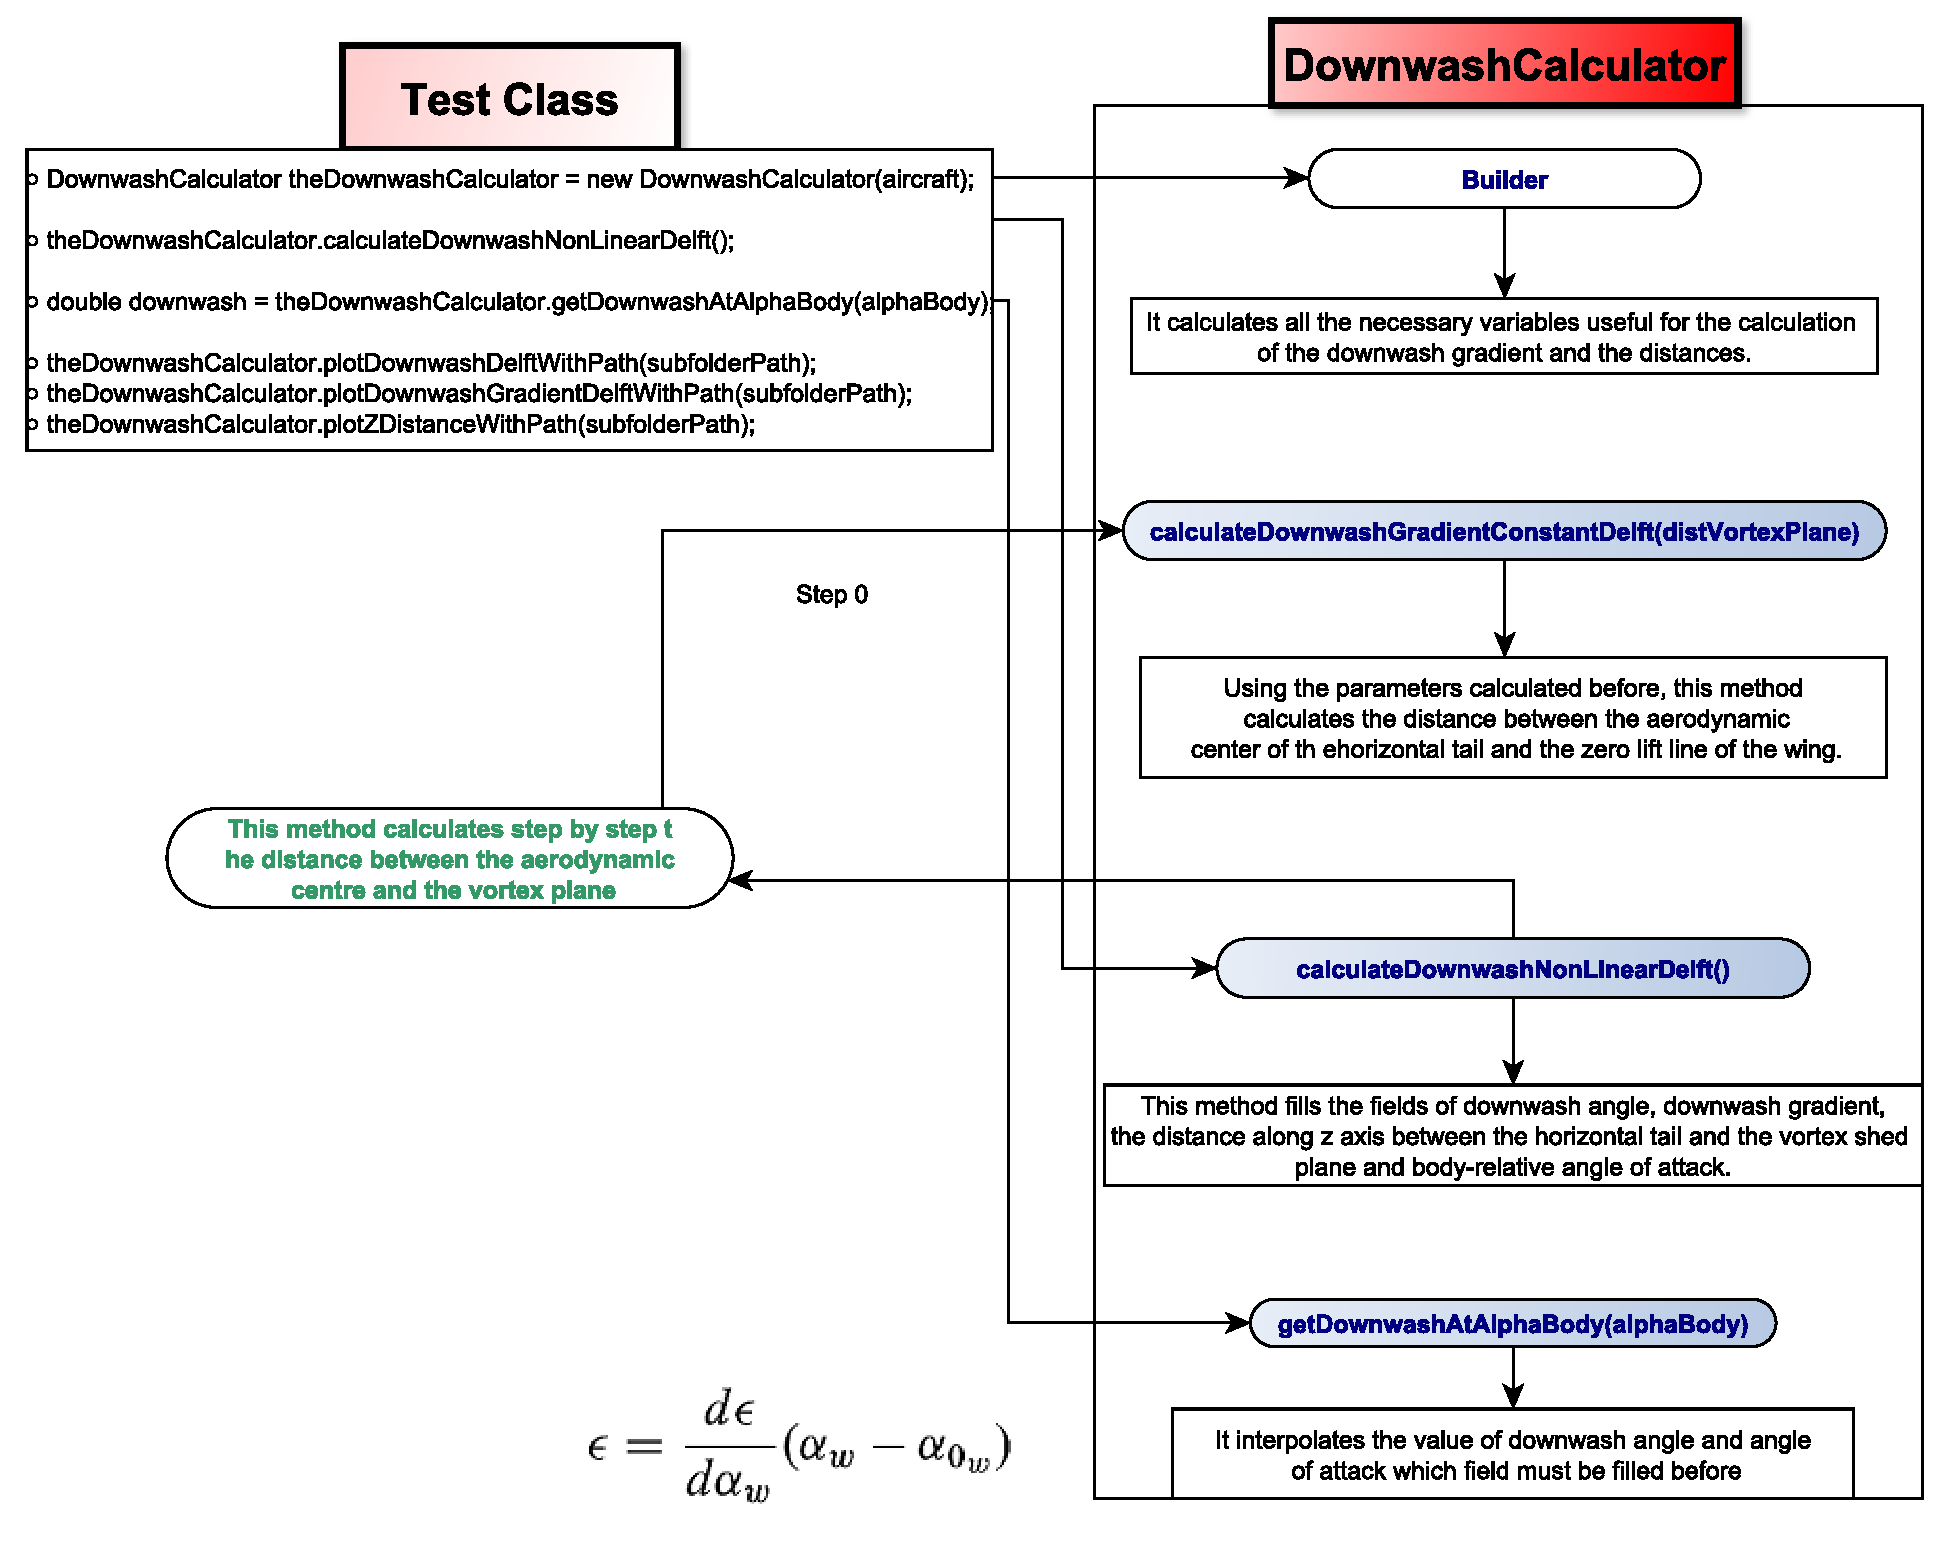
\includegraphics[height=13cm]{Immagini/nonlinear_2.pdf}} 
\caption{Flow chart of the calculation of non-linear downwash angle.}
\label{flowchartangles}
\end{figure} 


\section{Case Study}


\begin{lstlisting}[frame=rbl,caption={{\footnotesize Downwash Test Class}},label= [style=\bfseries]{Listing}]
	// -----------------------------------------------------------------------
	// INITIALIZE TEST CLASS ...
	// -----------------------------------------------------------------------

	// ------------------Downwash---------------

	System.out.println("\n-----Start of downwash calculation-----\n" );

	DownwashCalculator theDownwashCalculator = new DownwashCalculator(aircraft);
	
		theDownwashCalculator.calculateDownwashNonLinearDelft();
		
		theDownwashCalculator.plotDownwashDelftWithPath(subfolderPath);
		theDownwashCalculator.plotDownwashGradientDelftWithPath(subfolderPath);
		theDownwashCalculator.plotZDistanceWithPath(subfolderPath);
		theDownwashCalculator.plotXDistanceWithPath(subfolderPath);
	System.out.println(" DONE PLOTTING DOWNWASH ANGLE vs ALPHA BODY");

	double downwash = theDownwashCalculator.getDownwashAtAlphaBody(alphaBody);
	Amount<Angle> downwashAmountRadiant = Amount
					.valueOf(Math.toRadians(downwash), SI.RADIAN);
			System.out.println( "At alpha " + alphaBody
					.to(NonSI.DEGREE_ANGLE)
		.getEstimatedValue() + " (deg) the downwash angle is (deg) = " + downwash );
	}
}
\end{lstlisting}

In the previous listing is reported the Test Class used in order to evaluate the variability of the downwash gradient with $\alpha_B$. First of all the test class is initialized, after an Aircraft object is defined with the related analysis classes.

%import static java.lang.Math.toRadians;
%import java.io.File;
%import javax.measure.quantity.Angle;
%import javax.measure.unit.NonSI;
%import javax.measure.unit.SI;
%import org.jscience.physics.amount.Amount;
%import aircraft.OperatingConditions;
%import aircraft.calculators.ACAnalysisManager;
%import aircraft.components.Aircraft;
%import aircraft.components.liftingSurface.LSAerodynamicsManager;
%import aircraft.components.liftingSurface.LiftingSurface;
%import configuration.MyConfiguration;
%import configuration.enumerations.DatabaseReaderEnum;
%import javafx.util.Pair;
%import writers.JPADStaticWriteUtils;
%
%public class prova {
%
%    public static void main(String[] args) {
%	System.out.println("Initializing test class...");
%	String folderPath = MyConfiguration.currentDirectoryString + File.separator
%	                 + "out" + File.separator;
%	String subfolderPath = JPADStaticWriteUtils.createNewFolder(folderPath 
%	                 + "Longitudinal_Static_Stability" + File.separator);
%
%	//------------------------------------------------------------------------
%	// Default folders creation:
%
%	MyConfiguration.initWorkingDirectoryTree();
%
%	//------------------------------------------------------------------------
%	// Operating Condition 
%
%	OperatingConditions theConditions = new OperatingConditions();
%	theConditions.set_alphaCurrent(Amount.valueOf(toRadians(2.), SI.RADIAN));
%
%	//------------------------------------------------------------------------
%	// Default Aircraft 
%	Aircraft aircraft = Aircraft.createDefaultAircraft("ATR-72");
%	System.out.println("Default aircraft: " + aircraft.get_name() + "\n");
%
%	//------------------------------------------------------------------------
%	// Wing and Tail
%	LiftingSurface theWing = aircraft.get_wing();
%	LiftingSurface horizontalTail = aircraft.get_HTail();
%
%	//------------------------------------------------------------------------
%	// Aerodynamic managers
%	ACAnalysisManager theAnalysis = new ACAnalysisManager(theConditions);
%	theAnalysis.updateGeometry(aircraft);
%	LSAerodynamicsManager theLSAnalysis = new LSAerodynamicsManager(
%			theConditions, 
%			theWing,
%			aircraft
%			); 
%
%	aircraft.get_wing().setAerodynamics(theLSAnalysis);
%
%	aircraft.get_exposedWing().updateAirfoilsGeometryExposedWing( aircraft);
%	//------------------------------------------------------------------------
%	// Set databases
%	theLSAnalysis.setDatabaseReaders(
%			new Pair(DatabaseReaderEnum.AERODYNAMIC, 
%					"Aerodynamic_Database_Ultimate.h5"),
%			new Pair(DatabaseReaderEnum.HIGHLIFT,
%			"HighLiftDatabase.h5")
%			);	
%
%	//------------------------------------------------------------------------
%	// Angle of attack
%
%	Amount<Angle> alphaBody = theConditions.get_alphaCurrent();
%
%
%	// -----------------------------------------------------------------------
%	// LIFT CHARACTERISTICS 
%	// -----------------------------------------------------------------------
%
%	LSAerodynamicsManager.CalcCLAtAlpha theCLWingCalculator = theLSAnalysis
%	                     .new CalcCLAtAlpha();
%	                     
%	double cLIsolatedWing = theCLWingCalculator
%	                      .nasaBlackwellCompleteCurve(alphaBody);
\noindent\\
Below are the charts representing the results obtained by applying the method described at ATR 72 and BOEING 747-100B.

\subsection{ATR-72}

\begin{figure}[H]
\centering
%Disytance m Alpha Body 
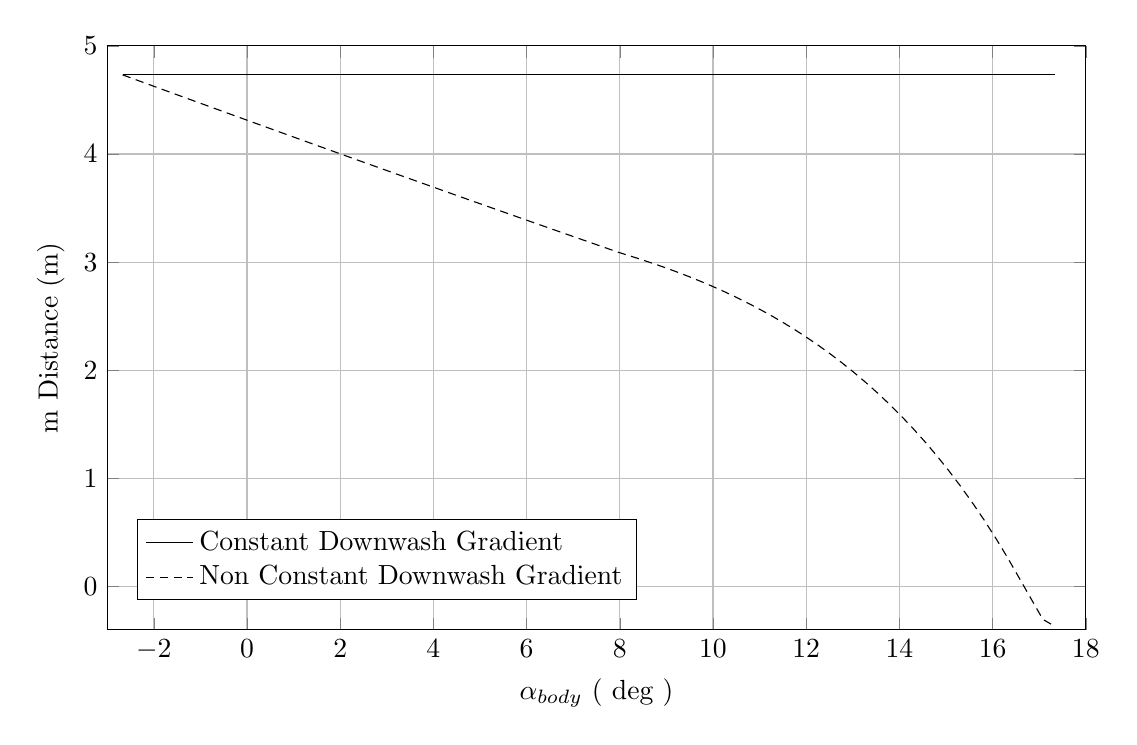
\begin{tikzpicture}

\begin{axis}[
width=14.01cm,
height=9cm,
scaled ticks=false, tick label style={/pgf/number format/fixed},
xmin=-3,
xmax=18,
xlabel={$\alpha_{body}$ ( deg )},
xmajorgrids,
ymin=-0.4,
ymax=5,
ylabel={m Distance (m)},
ymajorgrids,
legend style={at={(0.03,0.12)},anchor=west,draw=black,fill=white,legend cell align=left},
legend entries = {Constant Downwash Gradient\\Non Constant Downwash Gradient\\}
]

\addplot [
color=black,
solid
]
table[row sep=crcr]{
-2.6675212218928914	4.731135862150023\\
-2.4143566649308665	4.731135862150023\\
-2.1611921079688408	4.731135862150023\\
-1.9080275510068156	4.731135862150023\\
-1.6548629940447903	4.731135862150023\\
-1.401698437082765	4.731135862150023\\
-1.1485338801207396	4.731135862150023\\
-0.8953693231587143	4.731135862150023\\
-0.642204766196689	4.731135862150023\\
-0.38904020923466365	4.731135862150023\\
-0.13587565227263831	4.731135862150023\\
0.11728890468938702	4.731135862150023\\
0.37045346165141235	4.731135862150023\\
0.6236180186134377	4.731135862150023\\
0.8767825755754628	4.731135862150023\\
1.1299471325374886	4.731135862150023\\
1.3831116894995135	4.731135862150023\\
1.6362762464615384	4.731135862150023\\
1.8894408034235632	4.731135862150023\\
2.142605360385588	4.731135862150023\\
2.395769917347613	4.731135862150023\\
2.648934474309638	4.731135862150023\\
2.902099031271663	4.731135862150023\\
3.1552635882336877	4.731135862150023\\
3.4084281451957126	4.731135862150023\\
3.6615927021577375	4.731135862150023\\
3.9147572591197624	4.731135862150023\\
4.167921816081787	4.731135862150023\\
4.421086373043812	4.731135862150023\\
4.674250930005837	4.731135862150023\\
4.9274154869678615	4.731135862150023\\
5.180580043929886	4.731135862150023\\
5.433744600891911	4.731135862150023\\
5.686909157853936	4.731135862150023\\
5.940073714815961	4.731135862150023\\
6.193238271777986	4.731135862150023\\
6.446402828740011	4.731135862150023\\
6.699567385702036	4.731135862150023\\
6.952731942664061	4.731135862150023\\
7.2058964996260855	4.731135862150023\\
7.45906105658811	4.731135862150023\\
7.712225613550135	4.731135862150023\\
7.96539017051216	4.731135862150023\\
8.218554727474185	4.731135862150023\\
8.47171928443621	4.731135862150023\\
8.724883841398235	4.731135862150023\\
8.97804839836026	4.731135862150023\\
9.231212955322285	4.731135862150023\\
9.48437751228431	4.731135862150023\\
9.737542069246334	4.731135862150023\\
9.99070662620836	4.731135862150023\\
10.243871183170384	4.731135862150023\\
10.497035740132409	4.731135862150023\\
10.750200297094434	4.731135862150023\\
11.003364854056459	4.731135862150023\\
11.256529411018484	4.731135862150023\\
11.509693967980509	4.731135862150023\\
11.762858524942533	4.731135862150023\\
12.016023081904558	4.731135862150023\\
12.269187638866583	4.731135862150023\\
12.522352195828608	4.731135862150023\\
12.775516752790633	4.731135862150023\\
13.028681309752658	4.731135862150023\\
13.281845866714683	4.731135862150023\\
13.535010423676708	4.731135862150023\\
13.788174980638734	4.731135862150023\\
14.041339537600761	4.731135862150023\\
14.294504094562788	4.731135862150023\\
14.547668651524814	4.731135862150023\\
14.800833208486841	4.731135862150023\\
15.053997765448868	4.731135862150023\\
15.307162322410894	4.731135862150023\\
15.560326879372921	4.731135862150023\\
15.813491436334948	4.731135862150023\\
16.066655993296976	4.731135862150023\\
16.319820550259003	4.731135862150023\\
16.57298510722103	4.731135862150023\\
16.826149664183056	4.731135862150023\\
17.079314221145083	4.731135862150023\\
17.33247877810711	4.731135862150023\\
};

\addplot [
color=black,
densely dashed
]
table[row sep=crcr]{
-2.6675212218928914	4.731135862150023\\
-2.4143566649308665	4.69124387507764\\
-2.1611921079688408	4.651382837108132\\
-1.9080275510068156	4.6115537142831\\
-1.6548629940447903	4.571757459343794\\
-1.401698437082765	4.531995011609695\\
-1.1485338801207396	4.49226729686264\\
-0.8953693231587143	4.45257522723658\\
-0.642204766196689	4.4129197011129895\\
-0.38904020923466365	4.373301603022007\\
-0.13587565227263831	4.333721803549311\\
0.11728890468938702	4.294181159248802\\
0.37045346165141235	4.254680512561089\\
0.6236180186134377	4.2152206917378265\\
0.8767825755754628	4.175802510771899\\
1.1299471325374886	4.136426769333477\\
1.3831116894995135	4.097094252711948\\
1.6362762464615384	4.057805731763713\\
1.8894408034235632	4.018561962865861\\
2.142605360385588	3.979363687875674\\
2.395769917347613	3.9402116340959945\\
2.648934474309638	3.9011065142463868\\
2.902099031271663	3.862049026440091\\
3.1552635882336877	3.8230398541667214\\
3.4084281451957126	3.7840796662806815\\
3.6615927021577375	3.7451691169952435\\
3.9147572591197624	3.706308845882245\\
4.167921816081787	3.66749947787735\\
4.421086373043812	3.6287416232908143\\
4.674250930005837	3.5900358778237016\\
4.9274154869678615	3.5513828225894586\\
5.180580043929886	3.512783024140807\\
5.433744600891911	3.474237034501857\\
5.686909157853936	3.435745391205367\\
5.940073714815961	3.3973086173350717\\
6.193238271777986	3.358927221572983\\
6.446402828740011	3.320601698251579\\
6.699567385702036	3.2823325274107846\\
6.952731942664061	3.244120174859648\\
7.2058964996260855	3.2059650922426157\\
7.45906105658811	3.1678677171102954\\
7.712225613550135	3.1298284729946113\\
7.96539017051216	3.091847769488247\\
8.218554727474185	3.0576831590282074\\
8.47171928443621	3.022850759692497\\
8.724883841398235	2.986431931377665\\
8.97804839836026	2.948292300622619\\
9.231212955322285	2.9082967251303358\\
9.48437751228431	2.866306754881658\\
9.737542069246334	2.8221801834554587\\
9.99070662620836	2.7757705601893217\\
10.243871183170384	2.7269266607070195\\
10.497035740132409	2.675491912699894\\
10.750200297094434	2.621303773530386\\
11.003364854056459	2.5641930559270603\\
11.256529411018484	2.5039831977785734\\
11.509693967980509	2.4404894718294425\\
11.762858524942533	2.3735181309735895\\
12.016023081904558	2.3028654848748458\\
12.269187638866583	2.228316903881594\\
12.522352195828608	2.149645746733561\\
12.775516752790633	2.0666122094991226\\
13.028681309752658	1.9789620946850777\\
13.281845866714683	1.8864255017412483\\
13.535010423676708	1.7887154435070476\\
13.788174980638734	1.68552639788482\\
14.041339537600761	1.5765328106357284\\
14.294504094562788	1.4613875742846012\\
14.547668651524814	1.339720520446264\\
14.800833208486841	1.2111369793990534\\
15.053997765448868	1.0752164825644968\\
15.307162322410894	0.9315117120511347\\
15.560326879372921	0.7795478380592604\\
15.813491436334948	0.6188224311997208\\
16.066655993296976	0.44880619390130216\\
16.319820550259003	0.2689448235879794\\
16.57298510722103	0.07866239923375451\\
16.826149664183056	-0.11263522405853713\\
17.079314221145083	-0.3025679698832697\\
17.33247877810711	-0.36563982436565984\\
};
\end{axis}
\end{tikzpicture}%
\caption{ATR 72 Distance between AC horizontal tail and vortex plane vs $\alpha_{B}$.}
\label{fig:zATR}
\end{figure}
\noindent \\
\begin{figure}[H]
\centering
%Disytance m Alpha Body 
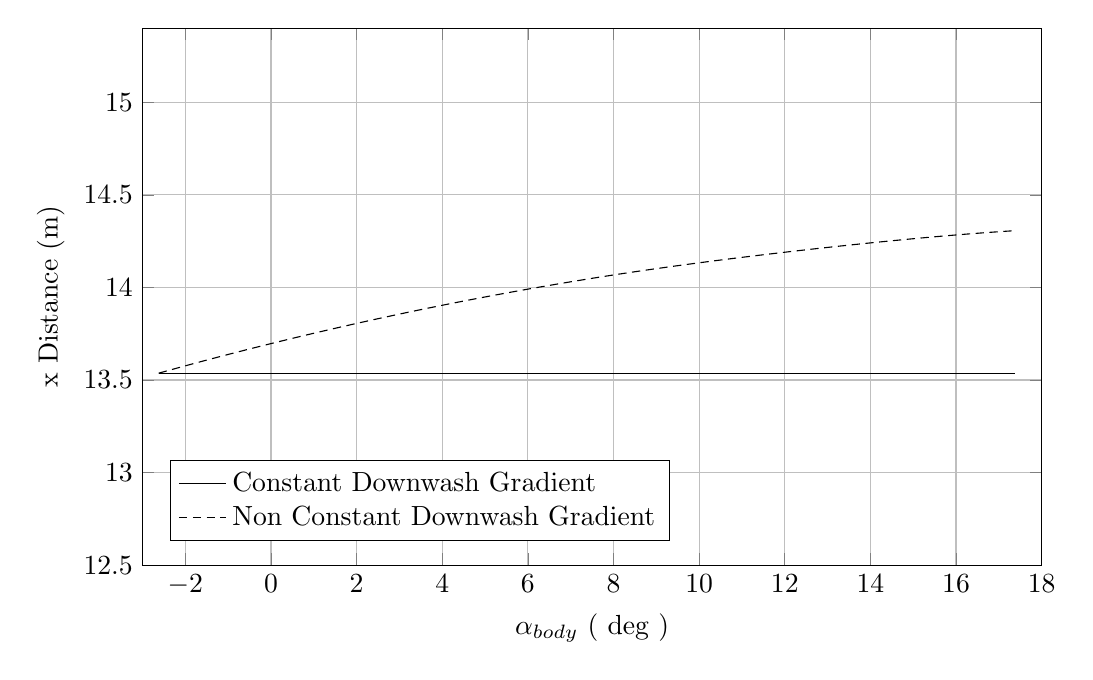
\begin{tikzpicture}

\begin{axis}[
width=13cm,
height=8.4cm,
scaled ticks=false, tick label style={/pgf/number format/fixed},
xmin=-3,
xmax=18,
xlabel={$\alpha_{body}$ ( deg )},
xmajorgrids,
ymin=12.5,
ymax=15.4,
ylabel={x Distance (m)},
ymajorgrids,
legend style={at={(0.03,0.12)},anchor=west,draw=black,fill=white,legend cell align=left},
legend entries = {Constant Downwash Gradient\\Non Constant Downwash Gradient\\}
]

\addplot [
color=black,
solid
]
table[row sep=crcr]{
-2.624111698071464	13.536683471822878\\
-2.370947141109438	13.536683471822878\\
-2.117782584147413	13.536683471822878\\
-1.8646180271853876	13.536683471822878\\
-1.6114534702233623	13.536683471822878\\
-1.358288913261337	13.536683471822878\\
-1.1051243562993116	13.536683471822878\\
-0.8519597993372863	13.536683471822878\\
-0.5987952423752609	13.536683471822878\\
-0.3456306854132356	13.536683471822878\\
-0.09246612845121027	13.536683471822878\\
0.16069842851081506	13.536683471822878\\
0.4138629854728404	13.536683471822878\\
0.6670275424348657	13.536683471822878\\
0.9201920993968908	13.536683471822878\\
1.1733566563589166	13.536683471822878\\
1.4265212133209415	13.536683471822878\\
1.6796857702829664	13.536683471822878\\
1.9328503272449913	13.536683471822878\\
2.186014884207016	13.536683471822878\\
2.439179441169041	13.536683471822878\\
2.692343998131066	13.536683471822878\\
2.945508555093091	13.536683471822878\\
3.1986731120551157	13.536683471822878\\
3.4518376690171406	13.536683471822878\\
3.7050022259791655	13.536683471822878\\
3.9581667829411904	13.536683471822878\\
4.211331339903215	13.536683471822878\\
4.46449589686524	13.536683471822878\\
4.717660453827265	13.536683471822878\\
4.97082501078929	13.536683471822878\\
5.223989567751315	13.536683471822878\\
5.47715412471334	13.536683471822878\\
5.730318681675365	13.536683471822878\\
5.9834832386373895	13.536683471822878\\
6.236647795599414	13.536683471822878\\
6.489812352561439	13.536683471822878\\
6.742976909523464	13.536683471822878\\
6.996141466485489	13.536683471822878\\
7.249306023447514	13.536683471822878\\
7.502470580409539	13.536683471822878\\
7.755635137371564	13.536683471822878\\
8.00879969433359	13.536683471822878\\
8.261964251295613	13.536683471822878\\
8.51512880825764	13.536683471822878\\
8.768293365219662	13.536683471822878\\
9.021457922181689	13.536683471822878\\
9.274622479143712	13.536683471822878\\
9.527787036105739	13.536683471822878\\
9.780951593067762	13.536683471822878\\
10.034116150029789	13.536683471822878\\
10.287280706991812	13.536683471822878\\
10.540445263953838	13.536683471822878\\
10.793609820915862	13.536683471822878\\
11.046774377877888	13.536683471822878\\
11.299938934839911	13.536683471822878\\
11.553103491801938	13.536683471822878\\
11.806268048763961	13.536683471822878\\
12.059432605725988	13.536683471822878\\
12.31259716268801	13.536683471822878\\
12.565761719650038	13.536683471822878\\
12.81892627661206	13.536683471822878\\
13.072090833574087	13.536683471822878\\
13.32525539053611	13.536683471822878\\
13.578419947498137	13.536683471822878\\
13.831584504460164	13.536683471822878\\
14.08474906142219	13.536683471822878\\
14.337913618384217	13.536683471822878\\
14.591078175346244	13.536683471822878\\
14.84424273230827	13.536683471822878\\
15.097407289270297	13.536683471822878\\
15.350571846232324	13.536683471822878\\
15.60373640319435	13.536683471822878\\
15.856900960156377	13.536683471822878\\
16.110065517118404	13.536683471822878\\
16.36323007408043	13.536683471822878\\
16.616394631042457	13.536683471822878\\
16.869559188004484	13.536683471822878\\
17.12272374496651	13.536683471822878\\
17.375888301928537	13.536683471822878\\
};

\addplot [
color=black,
densely dashed
]
table[row sep=crcr]{
-2.624111698071464	13.536683471822878\\
-2.370947141109438	13.552951292615692\\
-2.117782584147413	13.569038090917013\\
-1.8646180271853876	13.584944128611031\\
-1.6114534702233623	13.600669671000006\\
-1.358288913261337	13.61621498815194\\
-1.1051243562993116	13.631580354861246\\
-0.8519597993372863	13.646766050608543\\
-0.5987952423752609	13.661772359519682\\
-0.3456306854132356	13.676599570323923\\
-0.09246612845121027	13.69124797631132\\
0.16069842851081506	13.705717875289313\\
0.4138629854728404	13.720009569538513\\
0.6670275424348657	13.734123365767703\\
0.9201920993968908	13.748059575068073\\
1.1733566563589166	13.76181851286666\\
1.4265212133209415	13.775400498879051\\
1.6796857702829664	13.788805857061325\\
1.9328503272449913	13.802034915561233\\
2.186014884207016	13.81508800666866\\
2.439179441169041	13.827965466765377\\
2.692343998131066	13.840667636274048\\
2.945508555093091	13.853194859606552\\
3.1986731120551157	13.865547485111613\\
3.4518376690171406	13.877725865021757\\
3.7050022259791655	13.889730355399585\\
3.9581667829411904	13.901561316083404\\
4.211331339903215	13.913219110632221\\
4.46449589686524	13.924704106270102\\
4.717660453827265	13.936016673829915\\
4.97082501078929	13.94715718769649\\
5.223989567751315	13.958126025749166\\
5.47715412471334	13.968923569303811\\
5.730318681675365	13.979550203054247\\
5.9834832386373895	13.990006315013153\\
6.236647795599414	14.000292296452464\\
6.489812352561439	14.010408541843239\\
6.742976909523464	14.020355448795042\\
6.996141466485489	14.030133417994884\\
7.249306023447514	14.039742853145668\\
7.502470580409539	14.049184160904229\\
7.755635137371564	14.058457750818949\\
8.00879969433359	14.06756403526696\\
8.261964251295613	14.076473915470359\\
8.51512880825764	14.085180566287663\\
8.768293365219662	14.093710635864891\\
9.021457922181689	14.102068222655959\\
9.274622479143712	14.110266727134773\\
9.527787036105739	14.118309667445256\\
9.780951593067762	14.126207186997137\\
10.034116150029789	14.133964035610088\\
10.287280706991812	14.141587202011376\\
10.540445263953838	14.149082501293394\\
10.793609820915862	14.156453864655068\\
11.046774377877888	14.163707992146042\\
11.299938934839911	14.170845848842482\\
11.553103491801938	14.177874823060455\\
11.806268048763961	14.184793278243538\\
12.059432605725988	14.191608510505691\\
12.31259716268801	14.19831806848974\\
12.565761719650038	14.204926036890928\\
12.81892627661206	14.211430524604108\\
13.072090833574087	14.217832458706415\\
13.32525539053611	14.224130250182757\\
13.578419947498137	14.230321713743425\\
13.831584504460164	14.236405276814162\\
14.08474906142219	14.242375678423302\\
14.337913618384217	14.248231045485522\\
14.591078175346244	14.253963069113833\\
14.84424273230827	14.259569223322972\\
15.097407289270297	14.2650391180901\\
15.350571846232324	14.270367241913107\\
15.60373640319435	14.27554221751744\\
15.856900960156377	14.280554904312439\\
16.110065517118404	14.285392821808669\\
16.36323007408043	14.29004315613821\\
16.616394631042457	14.294491844471597\\
16.869559188004484	14.298722339895255\\
17.12272374496651	14.302718461554155\\
17.375888301928537	14.306459852967121\\
};
\end{axis}
\end{tikzpicture}%
\caption{ATR 72 distance between AC horizontal tail and AC of wing along the m direction vs $\alpha_{B}$.}
\label{fig:mATR}
\end{figure}


\begin{figure}[H]
\centering
%Downwash gradient vs Alpha Body NEW
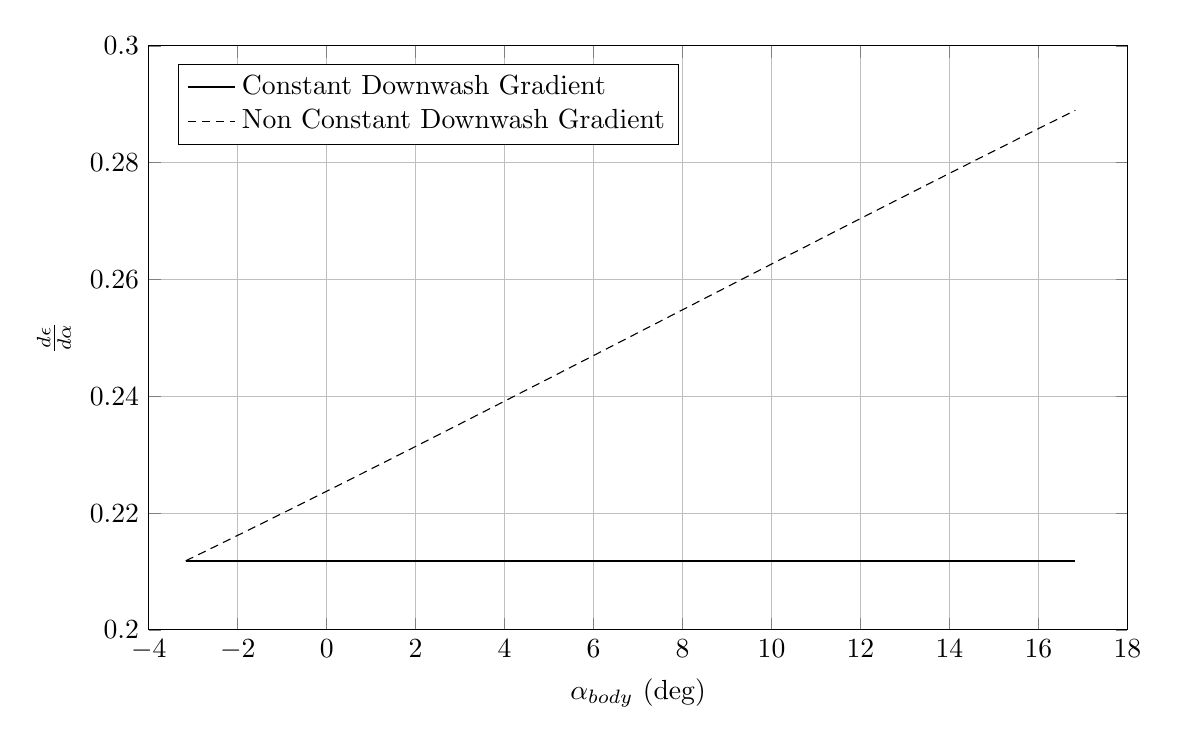
\begin{tikzpicture}

\begin{axis}[
width=14.01cm,
height=9cm,
scaled ticks=false, tick label style={/pgf/number format/fixed},
xmin=-4,
xmax=18,
xlabel={$\alpha_{body}$ (deg)},
xmajorgrids,
ymin=0.2,
ymax=0.3,
ylabel={$\frac{d \epsilon}{d \alpha}$ },
ymajorgrids,
legend style={at={(0.03,0.9)},anchor=west,draw=black,fill=white,legend cell align=left},
legend entries = {Constant Downwash Gradient\\Non Constant Downwash Gradient\\}
]

\addplot [
color=black,
thick
]
table[row sep=crcr]{
-3.169553350368967	0.21183320625402868\\
-2.9163887934069415	0.21183320625402868\\
-2.663224236444916	0.21183320625402868\\
-2.410059679482891	0.21183320625402868\\
-2.1568951225208655	0.21183320625402868\\
-1.9037305655588401	0.21183320625402868\\
-1.6505660085968148	0.21183320625402868\\
-1.3974014516347895	0.21183320625402868\\
-1.1442368946727641	0.21183320625402868\\
-0.8910723377107388	0.21183320625402868\\
-0.6379077807487135	0.21183320625402868\\
-0.3847432237866881	0.21183320625402868\\
-0.1315786668246628	0.21183320625402868\\
0.12158589013736254	0.21183320625402868\\
0.3747504470993879	0.21183320625402868\\
0.6279150040614132	0.21183320625402868\\
0.8810795610234385	0.21183320625402868\\
1.1342441179854634	0.21183320625402868\\
1.3874086749474883	0.21183320625402868\\
1.6405732319095132	0.21183320625402868\\
1.893737788871538	0.21183320625402868\\
2.146902345833563	0.21183320625402868\\
2.400066902795588	0.21183320625402868\\
2.6532314597576128	0.21183320625402868\\
2.906396016719637	0.21183320625402868\\
3.159560573681662	0.21183320625402868\\
3.412725130643687	0.21183320625402868\\
3.665889687605712	0.21183320625402868\\
3.9190542445677368	0.21183320625402868\\
4.172218801529762	0.21183320625402868\\
4.4253833584917865	0.21183320625402868\\
4.678547915453811	0.21183320625402868\\
4.931712472415836	0.21183320625402868\\
5.184877029377861	0.21183320625402868\\
5.438041586339886	0.21183320625402868\\
5.691206143301911	0.21183320625402868\\
5.944370700263936	0.21183320625402868\\
6.197535257225961	0.21183320625402868\\
6.450699814187986	0.21183320625402868\\
6.7038643711500105	0.21183320625402868\\
6.957028928112035	0.21183320625402868\\
7.21019348507406	0.21183320625402868\\
7.463358042036085	0.21183320625402868\\
7.71652259899811	0.21183320625402868\\
7.969687155960135	0.21183320625402868\\
8.22285171292216	0.21183320625402868\\
8.476016269884184	0.21183320625402868\\
8.72918082684621	0.21183320625402868\\
8.982345383808234	0.21183320625402868\\
9.23550994077026	0.21183320625402868\\
9.488674497732283	0.21183320625402868\\
9.74183905469431	0.21183320625402868\\
9.995003611656333	0.21183320625402868\\
10.24816816861836	0.21183320625402868\\
10.501332725580383	0.21183320625402868\\
10.75449728254241	0.21183320625402868\\
11.007661839504433	0.21183320625402868\\
11.26082639646646	0.21183320625402868\\
11.513990953428483	0.21183320625402868\\
11.76715551039051	0.21183320625402868\\
12.020320067352532	0.21183320625402868\\
12.273484624314559	0.21183320625402868\\
12.526649181276582	0.21183320625402868\\
12.779813738238609	0.21183320625402868\\
13.032978295200632	0.21183320625402868\\
13.286142852162659	0.21183320625402868\\
13.539307409124685	0.21183320625402868\\
13.792471966086712	0.21183320625402868\\
14.045636523048739	0.21183320625402868\\
14.298801080010765	0.21183320625402868\\
14.551965636972792	0.21183320625402868\\
14.805130193934819	0.21183320625402868\\
15.058294750896845	0.21183320625402868\\
15.311459307858872	0.21183320625402868\\
15.564623864820899	0.21183320625402868\\
15.817788421782925	0.21183320625402868\\
16.070952978744952	0.21183320625402868\\
16.32411753570698	0.21183320625402868\\
16.577282092669005	0.21183320625402868\\
16.830446649631032	0.21183320625402868\\
};

\addplot [
color=black,
densely dashed
]
table[row sep=crcr]{
-3.169553350368967	0.21183320625402868\\
-2.9163887934069415	0.21277220832857538\\
-2.663224236444916	0.21371363258684833\\
-2.410059679482891	0.21465742559910517\\
-2.1568951225208655	0.2156035334801616\\
-1.9037305655588401	0.21655190190587265\\
-1.6505660085968148	0.21750247612986656\\
-1.3974014516347895	0.21845520100051946\\
-1.1442368946727641	0.21941002097815557\\
-0.8910723377107388	0.22036688015245975\\
-0.6379077807487135	0.2213257222600863\\
-0.3847432237866881	0.22228649070245077\\
-0.1315786668246628	0.223249128563688\\
0.12158589013736254	0.22421357862876357\\
0.3747504470993879	0.2251797834017208\\
0.6279150040614132	0.22614768512405\\
0.8810795610234385	0.22711722579316368\\
1.1342441179854634	0.22808834718096105\\
1.3874086749474883	0.2290609908524691\\
1.6405732319095132	0.2300350981845411\\
1.893737788871538	0.23101061038460013\\
2.146902345833563	0.23198746850940938\\
2.400066902795588	0.23296561348385603\\
2.6532314597576128	0.23394498611973133\\
2.906396016719637	0.2349255271344935\\
3.159560573681662	0.2359071771699958\\
3.412725130643687	0.23688987681116752\\
3.665889687605712	0.23787356660463027\\
3.9190542445677368	0.2388581870772378\\
4.172218801529762	0.23984367875452164\\
4.4253833584917865	0.24082998217903084\\
4.678547915453811	0.24181703792855133\\
4.931712472415836	0.24280478663418992\\
5.184877029377861	0.24379316899831058\\
5.438041586339886	0.24478212581231037\\
5.691206143301911	0.24577159797422057\\
5.944370700263936	0.24676152650612254\\
6.197535257225961	0.24775185257136376\\
6.450699814187986	0.2487425174915651\\
6.7038643711500105	0.24973346276340555\\
6.957028928112035	0.25072463007517526\\
7.21019348507406	0.2517159613230841\\
7.463358042036085	0.2527073986273186\\
7.71652259899811	0.25369888434783416\\
7.969687155960135	0.2546903610998764\\
8.22285171292216	0.25568177176921986\\
8.476016269884184	0.2566730595271178\\
8.72918082684621	0.2576641678449536\\
8.982345383808234	0.2586550405085876\\
9.23550994077026	0.2596456216323908\\
9.488674497732283	0.26063585567295927\\
9.74183905469431	0.2616256874425042\\
9.995003611656333	0.26261506212190977\\
10.24816816861836	0.2636039252734554\\
10.501332725580383	0.2645922228531963\\
10.75449728254241	0.26557990122299874\\
11.007661839504433	0.26656690716222553\\
11.26082639646646	0.26755318787906845\\
11.513990953428483	0.268538691021525\\
11.76715551039051	0.2695233646880159\\
12.020320067352532	0.2705071574376418\\
12.273484624314559	0.2714900183000775\\
12.526649181276582	0.2724718967851024\\
12.779813738238609	0.273452742891765\\
13.032978295200632	0.2744325071171834\\
13.286142852162659	0.2754111404649787\\
13.539307409124685	0.2763885944533443\\
13.792471966086712	0.27736482112274924\\
14.045636523048739	0.2783397730432789\\
14.298801080010765	0.2793134033216125\\
14.551965636972792	0.2802856656076398\\
14.805130193934819	0.28125651410071995\\
15.058294750896845	0.2822259035555826\\
15.311459307858872	0.2831937892878761\\
15.564623864820899	0.28416012717936484\\
15.817788421782925	0.2851248736827785\\
16.070952978744952	0.28608798582631756\\
16.32411753570698	0.2870494212178181\\
16.577282092669005	0.2880091380485813\\
16.830446649631032	0.2889670950968686\\
};
\end{axis}
\end{tikzpicture}%

\caption{ATR 72 Downwash gradient vs $\alpha_{B}$.M=0.4}
\label{fig:downwashgradATR}
\end{figure}
\noindent \\\\
\begin{figure}[H]
\centering
%Epsilon vs Alpha Body NEW
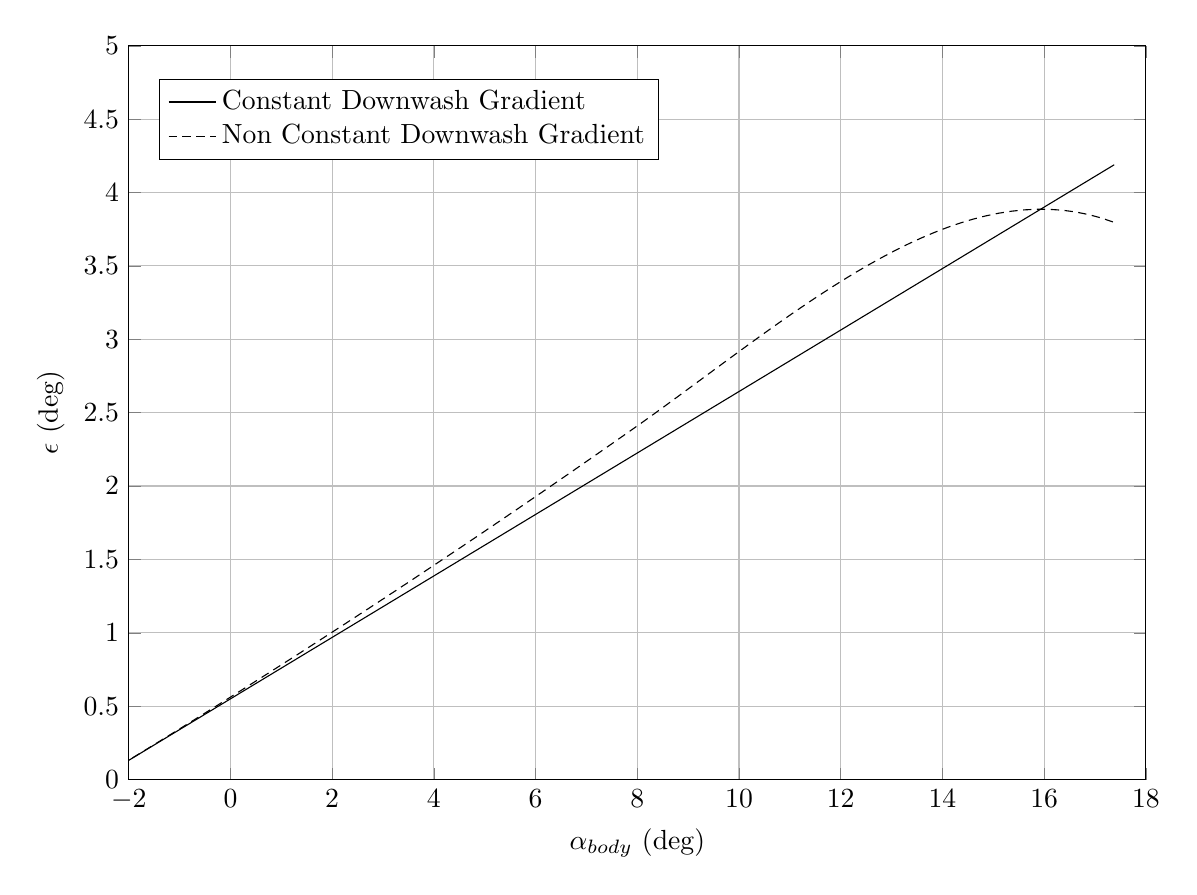
\begin{tikzpicture}

\begin{axis}[
width=14.5cm,
height=10.9cm,
scaled ticks=false, tick label style={/pgf/number format/fixed},
xmin=-2,
xmax=18,
xlabel={$\alpha_{body}$ (deg)},
xmajorgrids,
ymin=0,
ymax=5,
ylabel={$\epsilon$ (deg)},
ymajorgrids,
legend style={at={(0.03,0.9)},anchor=west,draw=black,fill=white,legend cell align=left},
legend entries = {Constant Downwash Gradient\\Non Constant Downwash Gradient\\}
]

\addplot [
color=black,
solid
]
table[row sep=crcr]{
-2.624111698071464	0.0\\
-2.370947141109438	0.0530276307304948\\
-2.117782584147413	0.1060552614609896\\
-1.8646180271853876	0.15908289219148442\\
-1.6114534702233623	0.2121105229219792\\
-1.358288913261337	0.265138153652474\\
-1.1051243562993116	0.31816578438296883\\
-0.8519597993372863	0.37119341511346365\\
-0.5987952423752609	0.4242210458439584\\
-0.3456306854132356	0.47724867657445325\\
-0.09246612845121027	0.530276307304948\\
0.16069842851081506	0.5833039380354429\\
0.4138629854728404	0.6363315687659377\\
0.6670275424348657	0.6893591994964324\\
0.9201920993968908	0.7423868302269273\\
1.1733566563589166	0.7954144609574221\\
1.4265212133209415	0.8484420916879168\\
1.6796857702829664	0.9014697224184116\\
1.9328503272449913	0.9544973531489063\\
2.186014884207016	1.007524983879401\\
2.439179441169041	1.0605526146098958\\
2.692343998131066	1.1135802453403905\\
2.945508555093091	1.1666078760708851\\
3.1986731120551157	1.2196355068013798\\
3.4518376690171406	1.2726631375318747\\
3.7050022259791655	1.3256907682623693\\
3.9581667829411904	1.378718398992864\\
4.211331339903215	1.4317460297233586\\
4.46449589686524	1.4847736604538533\\
4.717660453827265	1.5378012911843482\\
4.97082501078929	1.5908289219148428\\
5.223989567751315	1.6438565526453375\\
5.47715412471334	1.6968841833758321\\
5.730318681675365	1.749911814106327\\
5.9834832386373895	1.8029394448368217\\
6.236647795599414	1.8559670755673163\\
6.489812352561439	1.908994706297811\\
6.742976909523464	1.9620223370283059\\
6.996141466485489	2.0150499677588005\\
7.249306023447514	2.068077598489295\\
7.502470580409539	2.12110522921979\\
7.755635137371564	2.1741328599502845\\
8.00879969433359	2.227160490680779\\
8.261964251295613	2.2801881214112742\\
8.51512880825764	2.333215752141769\\
8.768293365219662	2.3862433828722636\\
9.021457922181689	2.439271013602758\\
9.274622479143712	2.492298644333253\\
9.527787036105739	2.5453262750637475\\
9.780951593067762	2.598353905794242\\
10.034116150029789	2.651381536524737\\
10.287280706991812	2.704409167255232\\
10.540445263953838	2.7574367979857266\\
10.793609820915862	2.8104644287162213\\
11.046774377877888	2.863492059446716\\
11.299938934839911	2.9165196901772106\\
11.553103491801938	2.9695473209077052\\
11.806268048763961	3.0225749516382\\
12.059432605725988	3.0756025823686945\\
12.31259716268801	3.1286302130991896\\
12.565761719650038	3.1816578438296843\\
12.81892627661206	3.234685474560179\\
13.072090833574087	3.2877131052906736\\
13.32525539053611	3.3407407360211683\\
13.578419947498137	3.393768366751663\\
13.831584504460164	3.446795997482158\\
14.08474906142219	3.499823628212653\\
14.337913618384217	3.5528512589431482\\
14.591078175346244	3.6058788896736433\\
14.84424273230827	3.6589065204041384\\
15.097407289270297	3.7119341511346335\\
15.350571846232324	3.7649617818651286\\
15.60373640319435	3.8179894125956237\\
15.856900960156377	3.871017043326119\\
16.110065517118404	3.924044674056614\\
16.36323007408043	3.977072304787109\\
16.616394631042457	4.030099935517604\\
16.869559188004484	4.083127566248099\\
17.12272374496651	4.136155196978594\\
17.375888301928537	4.1891828277090895\\
};

\addplot [
color=black,
densely dashed
]
table[row sep=crcr]{
-2.624111698071464	0.0\\
-2.370947141109438	0.05323062826185451\\
-2.117782584147413	0.1066608341861309\\
-1.8646180271853876	0.1602910971250473\\
-1.6114534702233623	0.21412188941138116\\
-1.358288913261337	0.26815367622450986\\
-1.1051243562993116	0.32238691545716025\\
-0.8519597993372863	0.376822057582922\\
-0.5987952423752609	0.4314595455245812\\
-0.3456306854132356	0.48629981452333043\\
-0.09246612845121027	0.5413432920089104\\
0.16069842851081506	0.5965903974707408\\
0.4138629854728404	0.6520415423300969\\
0.6670275424348657	0.7076971298133876\\
0.9201920993968908	0.7635575548265922\\
1.1733566563589166	0.8196232038309126\\
1.4265212133209415	0.8758944547196983\\
1.6796857702829664	0.9323716766966982\\
1.9328503272449913	0.9890552301556992\\
2.186014884207016	1.0459454665616046\\
2.439179441169041	1.1030427283330102\\
2.692343998131066	1.1603473487263334\\
2.945508555093091	1.21785965172155\\
3.1986731120551157	1.2755799519095958\\
3.4518376690171406	1.3335085543814837\\
3.7050022259791655	1.3916457546191952\\
3.9581667829411904	1.4499918383883958\\
4.211331339903215	1.5085470816330315\\
4.46449589686524	1.5673117503718543\\
4.717660453827265	1.6262861005969327\\
4.97082501078929	1.685470378174195\\
5.223989567751315	1.7448648187460598\\
5.47715412471334	1.8044696476361974\\
5.730318681675365	1.8642850797564778\\
5.9834832386373895	1.9243113195161479\\
6.236647795599414	1.9845485607332867\\
6.489812352561439	2.0449969865485857\\
6.742976909523464	2.105656769341498\\
6.996141466485489	2.166528070648798\\
7.249306023447514	2.227611041085601\\
7.502470580409539	2.288905820268877\\
7.755635137371564	2.3504125367435025\\
8.00879969433359	2.412131307910891\\
8.261964251295613	2.474699172001526\\
8.51512880825764	2.5383095634857495\\
8.768293365219662	2.6024212985581276\\
9.021457922181689	2.6669667495684566\\
9.274622479143712	2.7316572935812244\\
9.527787036105739	2.796415979662153\\
9.780951593067762	2.8610001168465518\\
10.034116150029789	2.925280345425107\\
10.287280706991812	2.9890605406668884\\
10.540445263953838	3.052158214764462\\
10.793609820915862	3.1144244073135106\\
11.046774377877888	3.175622732211913\\
11.299938934839911	3.2356519586513763\\
11.553103491801938	3.294220974856417\\
11.806268048763961	3.351268814142467\\
12.059432605725988	3.406464758771478\\
12.31259716268801	3.459736884936966\\
12.565761719650038	3.5108013899854362\\
12.81892627661206	3.559531383418669\\
13.072090833574087	3.6056904054467283\\
13.32525539053611	3.64909557345244\\
13.578419947498137	3.689558175474406\\
13.831584504460164	3.7268382329375283\\
14.08474906142219	3.76079516833161\\
14.337913618384217	3.7911307186049443\\
14.591078175346244	3.8177528137734846\\
14.84424273230827	3.8403036270106132\\
15.097407289270297	3.858698344437202\\
15.350571846232324	3.872601441490639\\
15.60373640319435	3.881881086558312\\
15.856900960156377	3.886248581057963\\
16.110065517118404	3.8855115109349434\\
16.36323007408043	3.879428268403375\\
16.616394631042457	3.8677443242006793\\
16.869559188004484	3.8502654331001205\\
17.12272374496651	3.8266733148648155\\
17.375888301928537	3.796821374773292\\
};
\end{axis}
\end{tikzpicture}%
\caption{ATR 72 Downwash angle vs $\alpha_{B}$. M=0.4.}
\label{fig:epsilon}
\end{figure}




\begin{lstlisting}[caption={{\footnotesize Downwash estimation - Results. ATR 72}},label= [style=\bfseries]{Listing}]
-----Start of downwash calculation-----

			DONE PLOTTING DOWNWASH ANGLE vs ALPHA BODY

At alpha 1.9999999999999996 (deg) the downwash angle is (deg) = 1.1242568216721218
-----------angles-------------- 
Angle of attack alpha body (deg) = 2.0
Angle of incidence of horizontal tail (deg) 0.0
Downwash Angle at Alpha Body (deg) 1.1242568216721218
Angle of Attack of Horizontal Tail (deg) 0.8757431783278777
\end{lstlisting}

\subsection{BOEING 747-100B}
\begin{figure}[H]
\centering
\input{immagini/mDistanceBOEING.tikz}
\caption{BOEING 747-100B Distance between AC horizontal tail and vortex plane vs $\alpha_{B}$.}
\label{fig:zATR}
\end{figure}
\noindent \\
\begin{figure}[H]
\centering
\input{immagini/zdistanceboeing.tikz}
\caption{BOEING 747-100B distance between AC horizontal tail and AC of wing along the m direction vs $\alpha_{B}$.}
\label{fig:zboeing}
\end{figure}


\begin{figure}[H]
\centering
%Downwash gradient vs Alpha Body NEW
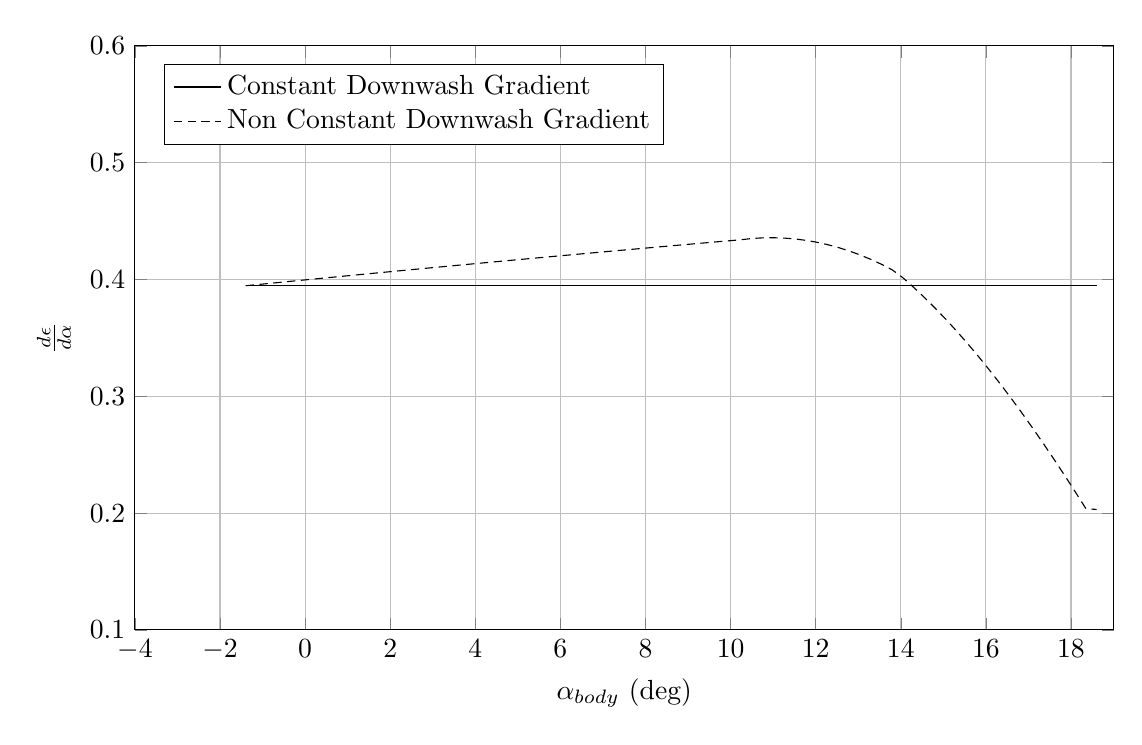
\begin{tikzpicture}

\begin{axis}[
width=14.01cm,
height=9cm,
scaled ticks=false, tick label style={/pgf/number format/fixed},
xmin=-4,
xmax=19,
xlabel={$\alpha_{body}$ (deg)},
xmajorgrids,
ymin=0.1,
ymax=0.6,
ylabel={$\frac{d \epsilon}{d \alpha}$ },
ymajorgrids,
legend style={at={(0.03,0.9)},anchor=west,draw=black,fill=white,legend cell align=left},
legend entries = {Constant Downwash Gradient\\Non Constant Downwash Gradient\\}
]

\addplot [
color=black,
solid
]
table[row sep=crcr]{
-1.3959898829117667	0.39462988423606277\\
-1.1428253259497414	0.39462988423606277\\
-0.8896607689877161	0.39462988423606277\\
-0.6364962120256907	0.39462988423606277\\
-0.3833316550636654	0.39462988423606277\\
-0.13016709810164007	0.39462988423606277\\
0.12299745886038527	0.39462988423606277\\
0.3761620158224106	0.39462988423606277\\
0.6293265727844359	0.39462988423606277\\
0.8824911297464613	0.39462988423606277\\
1.1356556867084866	0.39462988423606277\\
1.388820243670512	0.39462988423606277\\
1.6419848006325373	0.39462988423606277\\
1.8951493575945626	0.39462988423606277\\
2.1483139145565877	0.39462988423606277\\
2.4014784715186135	0.39462988423606277\\
2.6546430284806384	0.39462988423606277\\
2.9078075854426633	0.39462988423606277\\
3.160972142404688	0.39462988423606277\\
3.414136699366713	0.39462988423606277\\
3.667301256328738	0.39462988423606277\\
3.920465813290763	0.39462988423606277\\
4.173630370252788	0.39462988423606277\\
4.426794927214813	0.39462988423606277\\
4.6799594841768375	0.39462988423606277\\
4.933124041138862	0.39462988423606277\\
5.186288598100887	0.39462988423606277\\
5.439453155062912	0.39462988423606277\\
5.692617712024937	0.39462988423606277\\
5.945782268986962	0.39462988423606277\\
6.198946825948987	0.39462988423606277\\
6.452111382911012	0.39462988423606277\\
6.705275939873037	0.39462988423606277\\
6.9584404968350615	0.39462988423606277\\
7.211605053797086	0.39462988423606277\\
7.464769610759111	0.39462988423606277\\
7.717934167721136	0.39462988423606277\\
7.971098724683161	0.39462988423606277\\
8.224263281645186	0.39462988423606277\\
8.47742783860721	0.39462988423606277\\
8.730592395569236	0.39462988423606277\\
8.98375695253126	0.39462988423606277\\
9.236921509493285	0.39462988423606277\\
9.49008606645531	0.39462988423606277\\
9.743250623417335	0.39462988423606277\\
9.99641518037936	0.39462988423606277\\
10.249579737341385	0.39462988423606277\\
10.50274429430341	0.39462988423606277\\
10.755908851265435	0.39462988423606277\\
11.00907340822746	0.39462988423606277\\
11.262237965189485	0.39462988423606277\\
11.51540252215151	0.39462988423606277\\
11.768567079113534	0.39462988423606277\\
12.02173163607556	0.39462988423606277\\
12.274896193037584	0.39462988423606277\\
12.528060749999609	0.39462988423606277\\
12.781225306961634	0.39462988423606277\\
13.034389863923659	0.39462988423606277\\
13.287554420885684	0.39462988423606277\\
13.540718977847709	0.39462988423606277\\
13.793883534809734	0.39462988423606277\\
14.047048091771758	0.39462988423606277\\
14.300212648733783	0.39462988423606277\\
14.553377205695808	0.39462988423606277\\
14.806541762657833	0.39462988423606277\\
15.05970631961986	0.39462988423606277\\
15.312870876581886	0.39462988423606277\\
15.566035433543913	0.39462988423606277\\
15.81919999050594	0.39462988423606277\\
16.072364547467966	0.39462988423606277\\
16.325529104429993	0.39462988423606277\\
16.57869366139202	0.39462988423606277\\
16.831858218354046	0.39462988423606277\\
17.085022775316073	0.39462988423606277\\
17.3381873322781	0.39462988423606277\\
17.591351889240126	0.39462988423606277\\
17.844516446202153	0.39462988423606277\\
18.09768100316418	0.39462988423606277\\
18.350845560126206	0.39462988423606277\\
18.604010117088233	0.39462988423606277\\
};

\addplot [
color=black,
densely dashed
]
table[row sep=crcr]{
-1.3959898829117667	0.39462988423606277\\
-1.1428253259497414	0.3955408502459416\\
-0.8896607689877161	0.3964496444570807\\
-0.6364962120256907	0.3973562444020053\\
-0.3833316550636654	0.3982606281465814\\
-0.13016709810164007	0.39916277428617897\\
0.12299745886038527	0.400062661941695\\
0.3761620158224106	0.40096027075544194\\
0.6293265727844359	0.4018555808869094\\
0.8824911297464613	0.4027485730084043\\
1.1356556867084866	0.4036392283005749\\
1.388820243670512	0.4045275284478277\\
1.6419848006325373	0.40541345563363956\\
1.8951493575945626	0.4062969925357725\\
2.1483139145565877	0.40717812232139755\\
2.4014784715186135	0.408056828642133\\
2.6546430284806384	0.40893309562900015\\
2.9078075854426633	0.4098069078873067\\
3.160972142404688	0.41067825049145823\\
3.414136699366713	0.4115471089797059\\
3.667301256328738	0.41241346934883444\\
3.920465813290763	0.4132773180487957\\
4.173630370252788	0.4141386419772919\\
4.426794927214813	0.4149974284743142\\
4.6799594841768375	0.41585366531664003\\
4.933124041138862	0.41670734071229476\\
5.186288598100887	0.41755844329498165\\
5.439453155062912	0.4184069621184838\\
5.692617712024937	0.4192528866510419\\
5.945782268986962	0.420096206769714\\
6.198946825948987	0.4209369127547181\\
6.452111382911012	0.4217749952837629\\
6.705275939873037	0.42261044542637005\\
6.9584404968350615	0.42344325463819205\\
7.211605053797086	0.42427341475532726\\
7.464769610759111	0.42510091798863736\\
7.717934167721136	0.4259257569180692\\
7.971098724683161	0.42674792448698395\\
8.224263281645186	0.42756741399649745\\
8.47742783860721	0.42838421909983293\\
8.730592395569236	0.42919833379669153\\
8.98375695253126	0.4300097524276385\\
9.236921509493285	0.4308184696685137\\
9.49008606645531	0.4316244805248624\\
9.743250623417335	0.4324277803263939\\
9.99641518037936	0.4332283647214674\\
10.249579737341385	0.43402622967160664\\
10.50274429430341	0.43507027295892314\\
10.755908851265435	0.4356097880317553\\
11.00907340822746	0.43572258615272697\\
11.262237965189485	0.43540775597223813\\
11.51540252215151	0.4346642095323104\\
11.768567079113534	0.4334906357081423\\
12.02173163607556	0.4318854812386583\\
12.274896193037584	0.42984693149903674\\
12.528060749999609	0.4273728909799264\\
12.781225306961634	0.4244609634278081\\
13.034389863923659	0.4211084316040109\\
13.287554420885684	0.4173122366214698\\
13.540718977847709	0.4130689568235639\\
13.793883534809734	0.40837478617413325\\
14.047048091771758	0.4015306046047016\\
14.300212648733783	0.39331837477646847\\
14.553377205695808	0.38462991362235893\\
14.806541762657833	0.3754728742480702\\
15.05970631961986	0.36585514807383457\\
15.312870876581886	0.35578530876299447\\
15.566035433543913	0.3452726254797696\\
15.81919999050594	0.33432707218227503\\
16.072364547467966	0.3229593326797473\\
16.325529104429993	0.3111808009774018\\
16.57869366139202	0.2990035764452818\\
16.831858218354046	0.28644045337519275\\
17.085022775316073	0.273504904532621\\
17.3381873322781	0.260211058369371\\
17.591351889240126	0.24657366963928215\\
17.844516446202153	0.23260808325167062\\
18.09768100316418	0.21833019130622763\\
18.350845560126206	0.20375638337652452\\
18.604010117088233	0.2031367292757237\\
};
\end{axis}
\end{tikzpicture}%

\caption{BOEING 747-100B  Downwash gradient vs $\alpha_{B}$ .M=0.75.}
\label{fig:downwashgradboeing}
\end{figure}
\noindent \\ \\ 
\begin{figure}[H]
\centering
%Epsilon vs Alpha Body NEW
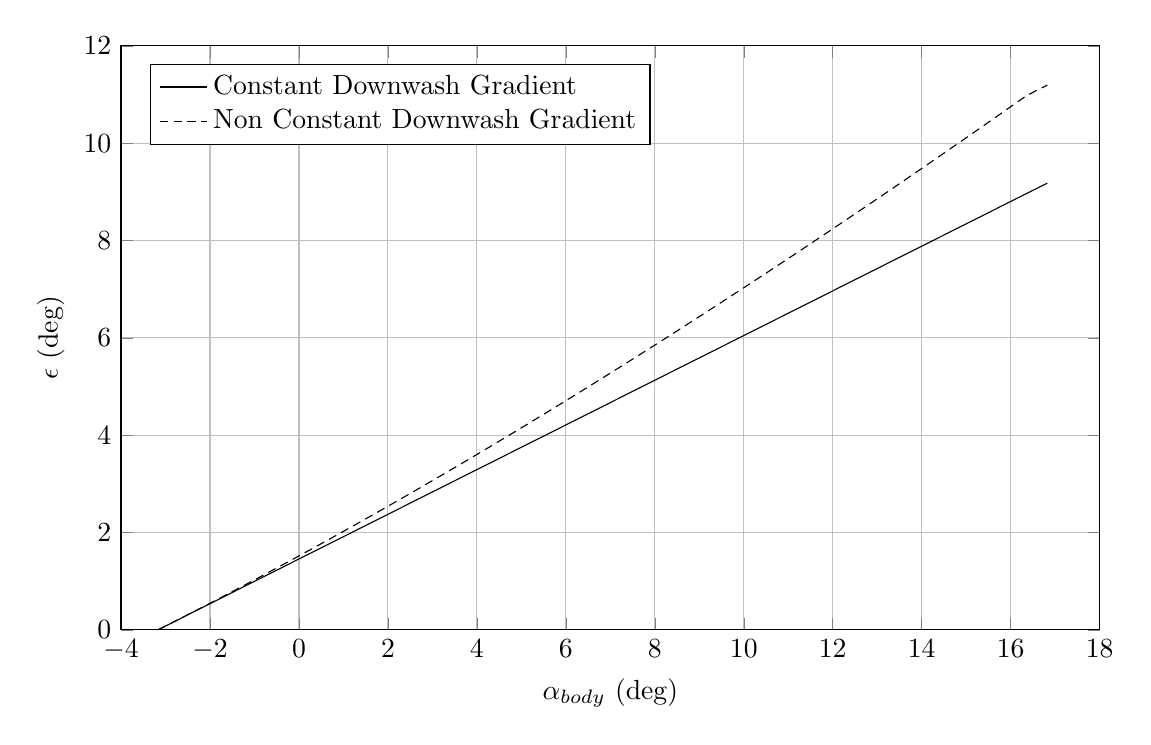
\begin{tikzpicture}

\begin{axis}[
width=14.01cm,
height=9cm,
scaled ticks=false, tick label style={/pgf/number format/fixed},
xmin=-4,
xmax=18,
xlabel={$\alpha_{body}$ (deg)},
xmajorgrids,
ymin=0.0,
ymax=12,
ylabel={$\epsilon$ (deg)},
ymajorgrids,
legend style={at={(0.03,0.9)},anchor=west,draw=black,fill=white,legend cell align=left},
legend entries = {Constant Downwash Gradient\\Non Constant Downwash Gradient\\}
]

\addplot [
color=black,
solid
]
table[row sep=crcr]{
-3.174711619549805	0.0\\
-2.9215470625877797	0.11620940723488471\\
-2.6683825056257544	0.23241881446976964\\
-2.415217948663729	0.34862822170465435\\
-2.1620533917017037	0.4648376289395393\\
-1.9088888347396784	0.5810470361744241\\
-1.655724277777653	0.6972564434093089\\
-1.4025597208156277	0.8134658506441937\\
-1.1493951638536024	0.9296752578790786\\
-0.8962306068915771	1.0458846651139633\\
-0.6430660499295517	1.1620940723488482\\
-0.3899014929675264	1.278303479583733\\
-0.13673693600550108	1.3945128868186178\\
0.11642762095652426	1.5107222940535026\\
0.3695921779185496	1.6269317012883875\\
0.6227567348805749	1.7431411085232722\\
0.8759212918426003	1.8593505157581571\\
1.1290858488046251	1.9755599229930416\\
1.38225040576665	2.091769330227926\\
1.635414962728675	2.207978737462811\\
1.8885795196906998	2.3241881446976955\\
2.1417440766527247	2.4403975519325805\\
2.3949086336147496	2.556606959167465\\
2.6480731905767745	2.6728163664023494\\
2.901237747538799	2.789025773637234\\
3.154402304500824	2.9052351808721184\\
3.4075668614628487	3.021444588107003\\
3.6607314184248736	3.137653995341888\\
3.9138959753868985	3.2538634025767723\\
4.167060532348923	3.3700728098116572\\
4.420225089310948	3.4862822170465417\\
4.673389646272973	3.602491624281426\\
4.926554203234998	3.7187010315163107\\
5.179718760197023	3.8349104387511956\\
5.432883317159048	3.95111984598608\\
5.686047874121073	4.067329253220965\\
5.939212431083098	4.183538660455849\\
6.1923769880451225	4.299748067690734\\
6.445541545007147	4.4159574749256185\\
6.698706101969172	4.532166882160503\\
6.951870658931197	4.648376289395388\\
7.205035215893222	4.764585696630272\\
7.458199772855247	4.880795103865157\\
7.711364329817272	4.997004511100042\\
7.964528886779297	5.113213918334926\\
8.217693443741322	5.229423325569811\\
8.470858000703346	5.345632732804695\\
8.724022557665371	5.46184214003958\\
8.977187114627396	5.578051547274465\\
9.230351671589421	5.69426095450935\\
9.483516228551446	5.810470361744234\\
9.736680785513471	5.926679768979119\\
9.989845342475496	6.042889176214003\\
10.24300989943752	6.159098583448888\\
10.496174456399546	6.275307990683772\\
10.74933901336157	6.3915173979186575\\
11.002503570323595	6.507726805153542\\
11.25566812728562	6.6239362123884264\\
11.508832684247645	6.740145619623311\\
11.76199724120967	6.856355026858195\\
12.015161798171695	6.97256443409308\\
12.26832635513372	7.088773841327964\\
12.521490912095745	7.20498324856285\\
12.77465546905777	7.321192655797734\\
13.027820026019794	7.437402063032619\\
13.280984582981821	7.553611470267504\\
13.534149139943848	7.6698208775023895\\
13.787313696905874	7.786030284737275\\
14.040478253867901	7.90223969197216\\
14.293642810829928	8.018449099207047\\
14.546807367791954	8.13465850644193\\
14.799971924753981	8.250867913676817\\
15.053136481716008	8.3670773209117\\
15.306301038678034	8.483286728146588\\
15.559465595640061	8.599496135381473\\
15.812630152602088	8.715705542616359\\
16.065794709564116	8.831914949851246\\
16.318959266526143	8.94812435708613\\
16.57212382348817	9.064333764321017\\
16.825288380450196	9.1805431715559\\
};

\addplot [
color=black,
densely dashed
]
table[row sep=crcr]{
-3.174711619549805	0.0\\
-2.9215470625877797	0.11662641233096166\\
-2.6683825056257544	0.2340825889306938\\
-2.415217948663729	0.3523621389476879\\
-2.1620533917017037	0.4714586452147729\\
-1.9088888347396784	0.5913656678717014\\
-1.655724277777653	0.7120767478755868\\
-1.4025597208156277	0.8335854103995118\\
-1.1493951638536024	0.9558851681198353\\
-0.8962306068915771	1.0789695243928956\\
-0.6430660499295517	1.2028319763220001\\
-0.3899014929675264	1.3274660177157287\\
-0.13673693600550108	1.4528651419387424\\
0.11642762095652426	1.5790228446564083\\
0.3695921779185496	1.7059326264746888\\
0.6227567348805749	1.8335879954768433\\
0.8759212918426003	1.9619824696585975\\
1.1290858488046251	2.0911095792635184\\
1.38225040576665	2.2209628690204264\\
1.635414962728675	2.3515359002847314\\
1.8885795196906998	2.482822253085649\\
2.1417440766527247	2.614815528081318\\
2.3949086336147496	2.7475093484238484\\
2.6480731905767745	2.88089736153642\\
2.901237747538799	3.0149732408045335\\
3.154402304500824	3.1497306871835673\\
3.4075668614628487	3.2851634307247983\\
3.6607314184248736	3.421265232022071\\
3.9138959753868985	3.55802988358128\\
4.167060532348923	3.6954512111148494\\
4.420225089310948	3.8335230747634026\\
4.673389646272973	3.972239370246754\\
4.926554203234998	4.111594029946414\\
5.179718760197023	4.251581023921726\\
5.432883317159048	4.392194360861741\\
5.686047874121073	4.5334280889749685\\
5.939212431083098	4.675276296819016\\
6.1923769880451225	4.817733114072208\\
6.445541545007147	4.9607927122491615\\
6.698706101969172	5.104449305362309\\
6.951870658931197	5.248697150531328\\
7.205035215893222	5.393530548542343\\
7.458199772855247	5.538943844358818\\
7.711364329817272	5.684931427585942\\
7.964528886779297	5.8314877328903\\
8.217693443741322	5.978607240376609\\
8.470858000703346	6.126284475923185\\
8.724022557665371	6.274514011477866\\
8.977187114627396	6.423290465315966\\
9.230351671589421	6.572608502261884\\
9.483516228551446	6.722462833875891\\
9.736680785513471	6.8728482186076185\\
9.989845342475496	7.023759461917678\\
10.24300989943752	7.175191416368853\\
10.496174456399546	7.3271389816882415\\
10.74933901336157	7.479597104801659\\
11.002503570323595	7.632560779841641\\
11.25566812728562	7.786025048130232\\
11.508832684247645	7.939984998137857\\
11.76199724120967	8.094435765419373\\
12.015161798171695	8.249372532528493\\
12.26832635513372	8.404790528911661\\
12.521490912095745	8.560685030782405\\
12.77465546905777	8.71705136097727\\
13.027820026019794	8.873884888794233\\
13.280984582981821	9.03118102981461\\
13.534149139943848	9.18893524570936\\
13.787313696905874	9.347143044030657\\
14.040478253867901	9.505799977989591\\
14.293642810829928	9.664901646220825\\
14.546807367791954	9.824443692534992\\
14.799971924753981	9.984421805659572\\
15.053136481716008	10.14483171896903\\
15.306301038678034	10.305669210204845\\
15.559465595640061	10.466930101186149\\
15.812630152602088	10.628610257511607\\
16.065794709564116	10.790705588253191\\
16.318959266526143	10.953212045642355\\
16.57212382348817	11.079410903101211\\
16.825288380450196	11.192825270921674\\
};
\end{axis}
\end{tikzpicture}%

\caption{BOEING 747-100B Downwash angle vs $\alpha_{B}$. M=0.75.}
\label{fig:epsilonboeing}
\end{figure}





\newpage

\begin{lstlisting}[caption={{\footnotesize Downwash estimation - Results. BOEING 747-100B}},label= [style=\bfseries]{Listing}]

-----Start of downwash calculation-----

			DONE PLOTTING DOWNWASH ANGLE vs ALPHA BODY

At alpha 1.9999999999999996 (deg) the downwash angle is (deg) = 2.540913931771228

 
-----------angles-------------- 
Angle of attack alpha body (deg) = 2.0
Angle of incidence of horizontal tail (deg) -0.9999999999999998
Downwash Angle at Alpha Body (deg) 1.3810738944458758
Angle of Attack of Horizontal Tail (deg) -0.381073894445876
\end{lstlisting}

\section{Results Comparison}

In order to compare the achieved results three methods of downwash estimation have been implemented in Microsoft Excel using ATR 72 data. The distances are obtained using the explained method, while the equation are expressed in the following sections.



\begin{figure}[H]
	\centering
{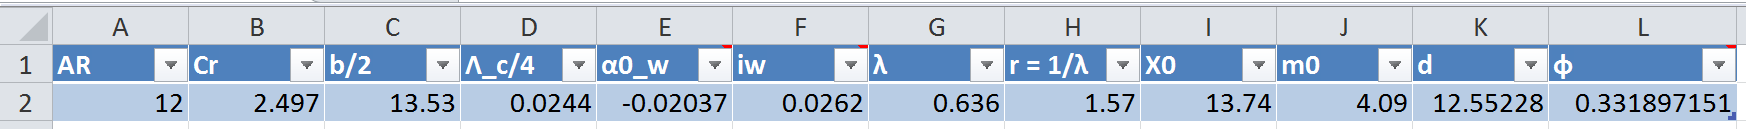
\includegraphics[height=1.1cm]{Immagini/datadownwash.png}} 
	\caption{Useful data for the downwash estimation.}
	\label{usefuldata}
\end{figure}

\subsection {Slingerland Method }

This is the method explained in the previous sections and this is the method that has been implemented in JPAD. This method has been presented in a master thesis by Mr. R. Slingerland, in TU Delft University.In order to evaluate the downwash, a model has been developed that computes the lift, drag and pitching moment in ground effect, utilizing Prandtl's lifting-line theory. As a by-product also the downwash in free air at the tail is determined. This model is innovative in the sense that it uses closed form expressions to include the vortex sheet relaxation, wing sweep and dihedral, the interaction of the wing- and flap vortices and the contribution of the rear fuselage-mounted nacelles. The equation presented in the relative section is valid also for sweeped wing.

\begin{figure}[H]
\centering
{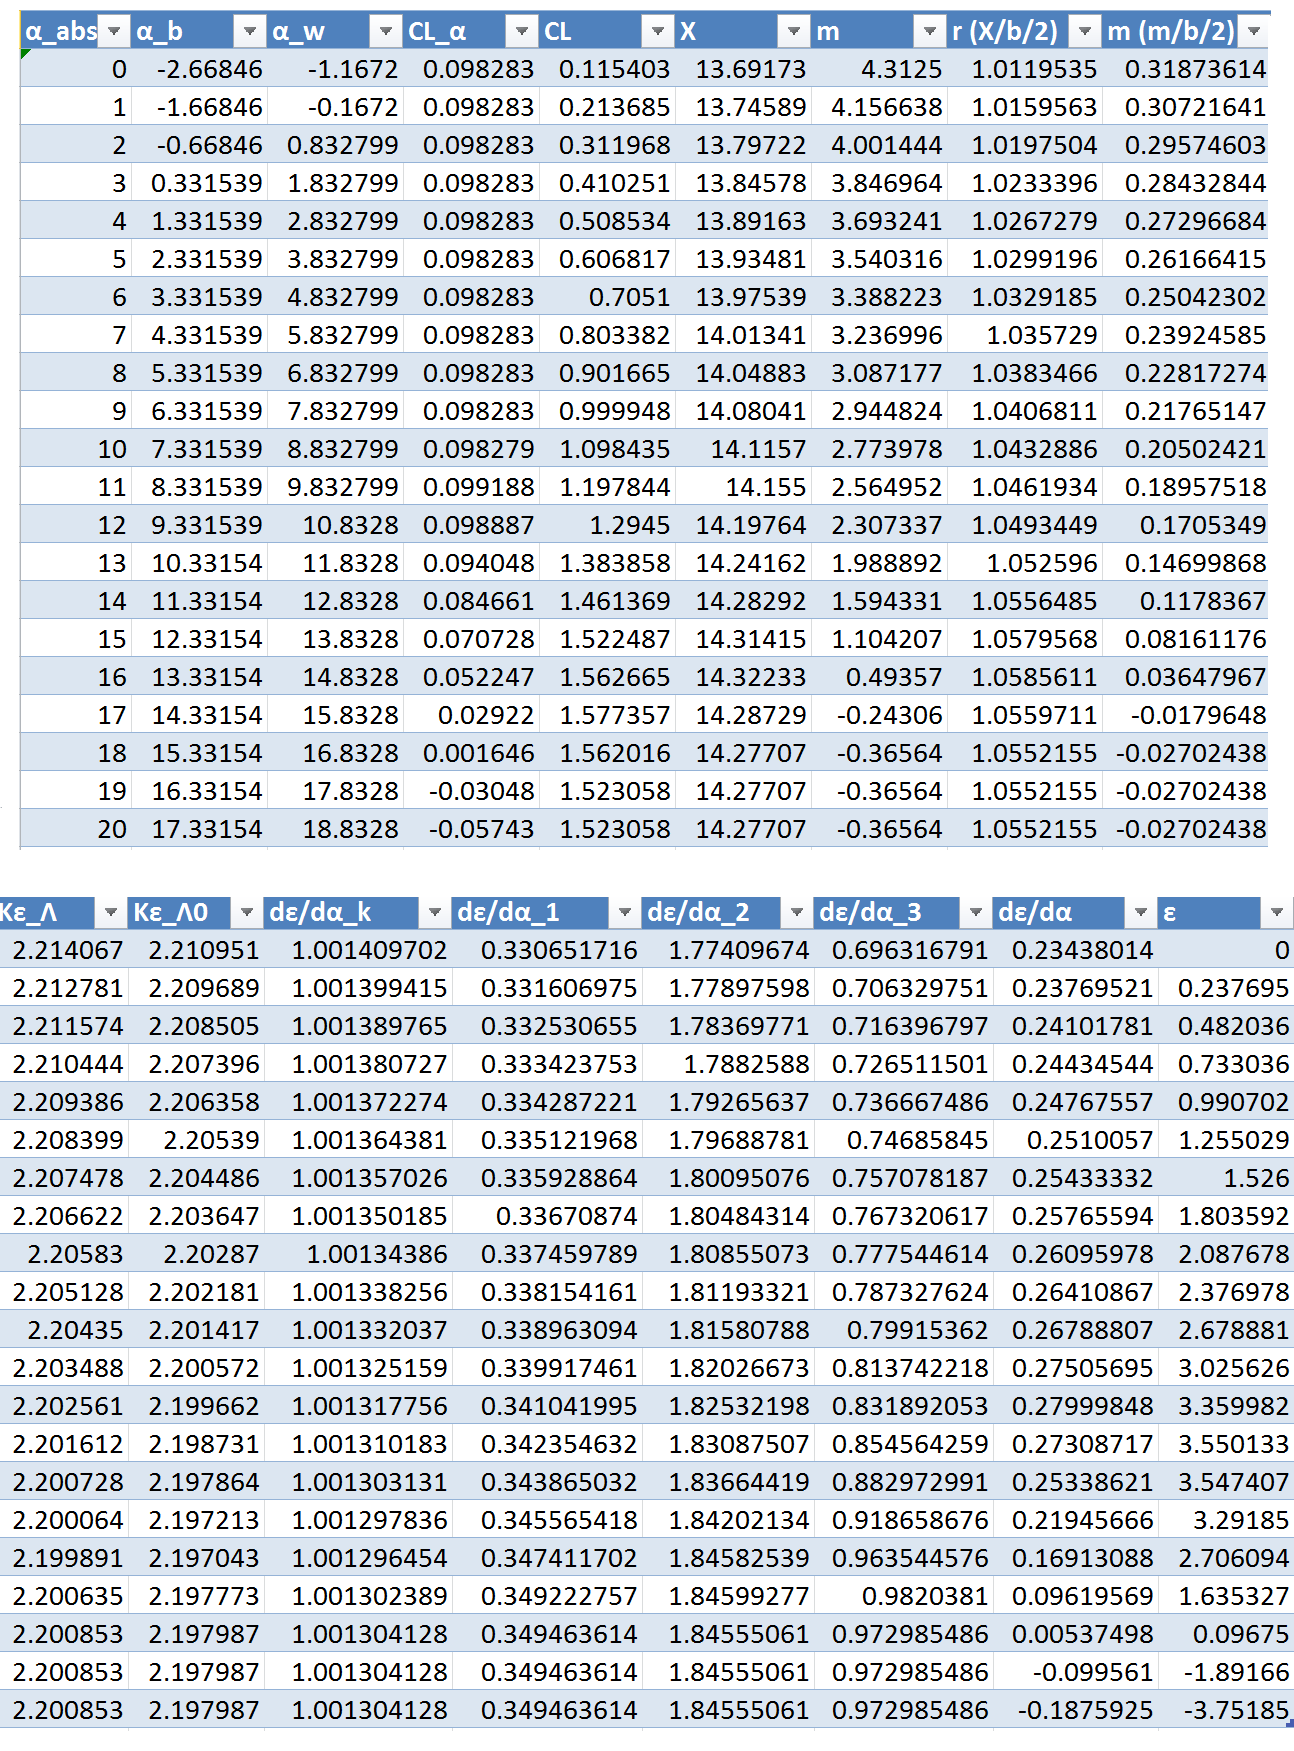
\includegraphics[height=7cm]{immagini/delft}} 
\label{delftdata}
\end{figure} 
\begin{figure}[H]
\centering
{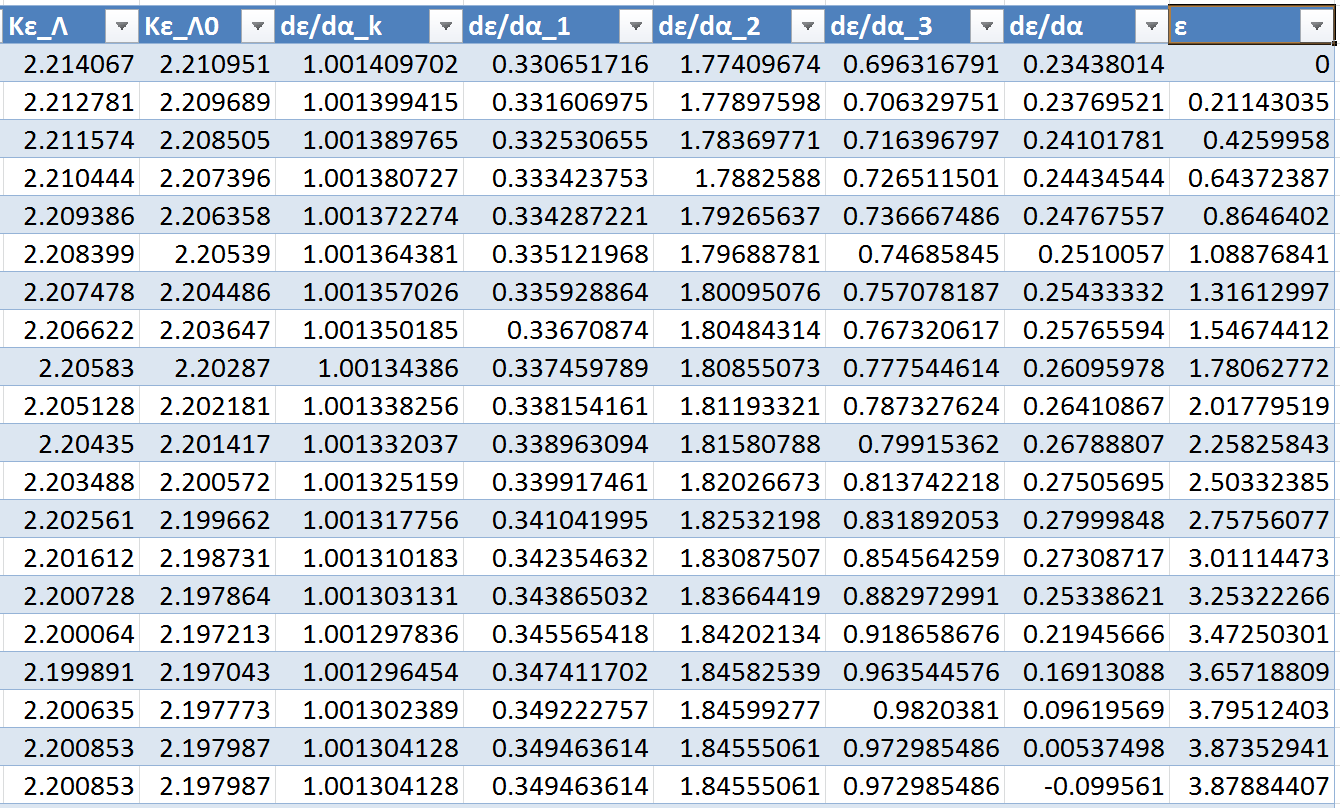
\includegraphics[height=7cm]{immagini/delftdata}} 
\caption{Data used for the calculation of downwash using Delft method.}
\label{delftdata}
\end{figure} 


\subsection {NACA Modified Method }
This method has been explained by Prof. Vincenzo Giordano\cite{uninagiordano}  based on the results obtained in NACA Report -648 \cite{Jacobs:NACA:Rep:648}.
The downwash behind a wing is mainly a function of the wing loading and is a manifestation of the associated vortex system. A first approximation to the downwash is obtained by assuming the sheet to originate at the quarter-chord line and to extend unchanged indefinitely downstream, the vortex system thereby consisting of elementary U-vortices (or horseshoe vorticcs). The actual sheet, however, does not extend unaltered from the lifting line to infinity because, as a result of the air motions that the vortex system itself creates, it is rapidly displaced downward and deformed. Inasmuch as the downwash depends to a predominant extent on the trailing vortex sheet, a vertical displacement of the sheet causes a vertical displacement of the entire downwash pattern by the same amount. \\ \\
This method introduces a function $\Phi$ useful in order to evaluate the downwash gradient and the downwash angle.
\begin{equation}
\Phi = \Phi ( \AR , \lambda, \alpha)
\end{equation}
Starting from this function it is possible to evaluate the downwash gradient as follows:
\begin{equation}
\frac{d\epsilon}{d \alpha } = C_{L_{\alpha}} \Phi + C_L \frac{d\Phi}{d \alpha }
\end{equation}
The value of $\Phi$ is obtained from charts fixed the $\AR$ and $\lambda$. The process is explained following.
\noindent \\

\begin{enumerate}
	\item An array of absolute angle of attack is defined
	\item Each value of $\alpha_a$ corresponds to an angle $\alpha_b$ and to an angle $\alpha_w$
	\item For each $\alpha$ is calculated the value of the lift coefficient curve slope
	\item The relative value of $C_L$ is calculated
	\item Using the geometrical construction introduced before the distances ``m'' and ``x'' is calculated
	\item Consequently the percentages distances ``$\frac{m}{\frac{b}{2}} 100$'' and ``$\frac{x}{\frac{b}{2}} 100$'' is calculated
	\item With the obtained value of ``x'' it is possible to enter in a chart that are parametrized for ``x'', ``m'' and $\lambda$ value. There are three charts for $x=70$, $x=80$, $x=90$. If the obtained value is not between these it is possible to do a linear interpolation
	\item For each value of $\AR$\ and ``x'' there are four curves in a chart that corresponding to different values of ``m''. The first curve represents the value of ``m'' for which the plan is in the slipstream. The other curves differ from the first one for $m \pm 10$. It's necessary to obtain the value of $\Phi$ corresponding to the real value of  ``m''.
\end{enumerate}

Known the value of the dowhwash gradient for each angle of attack it's possible to evaluate the angle of downwash

\begin{equation}
\epsilon = \frac{d\epsilon}{d\alpha} \alpha_a
\end{equation}
\begin{figure}[H]
\centering
{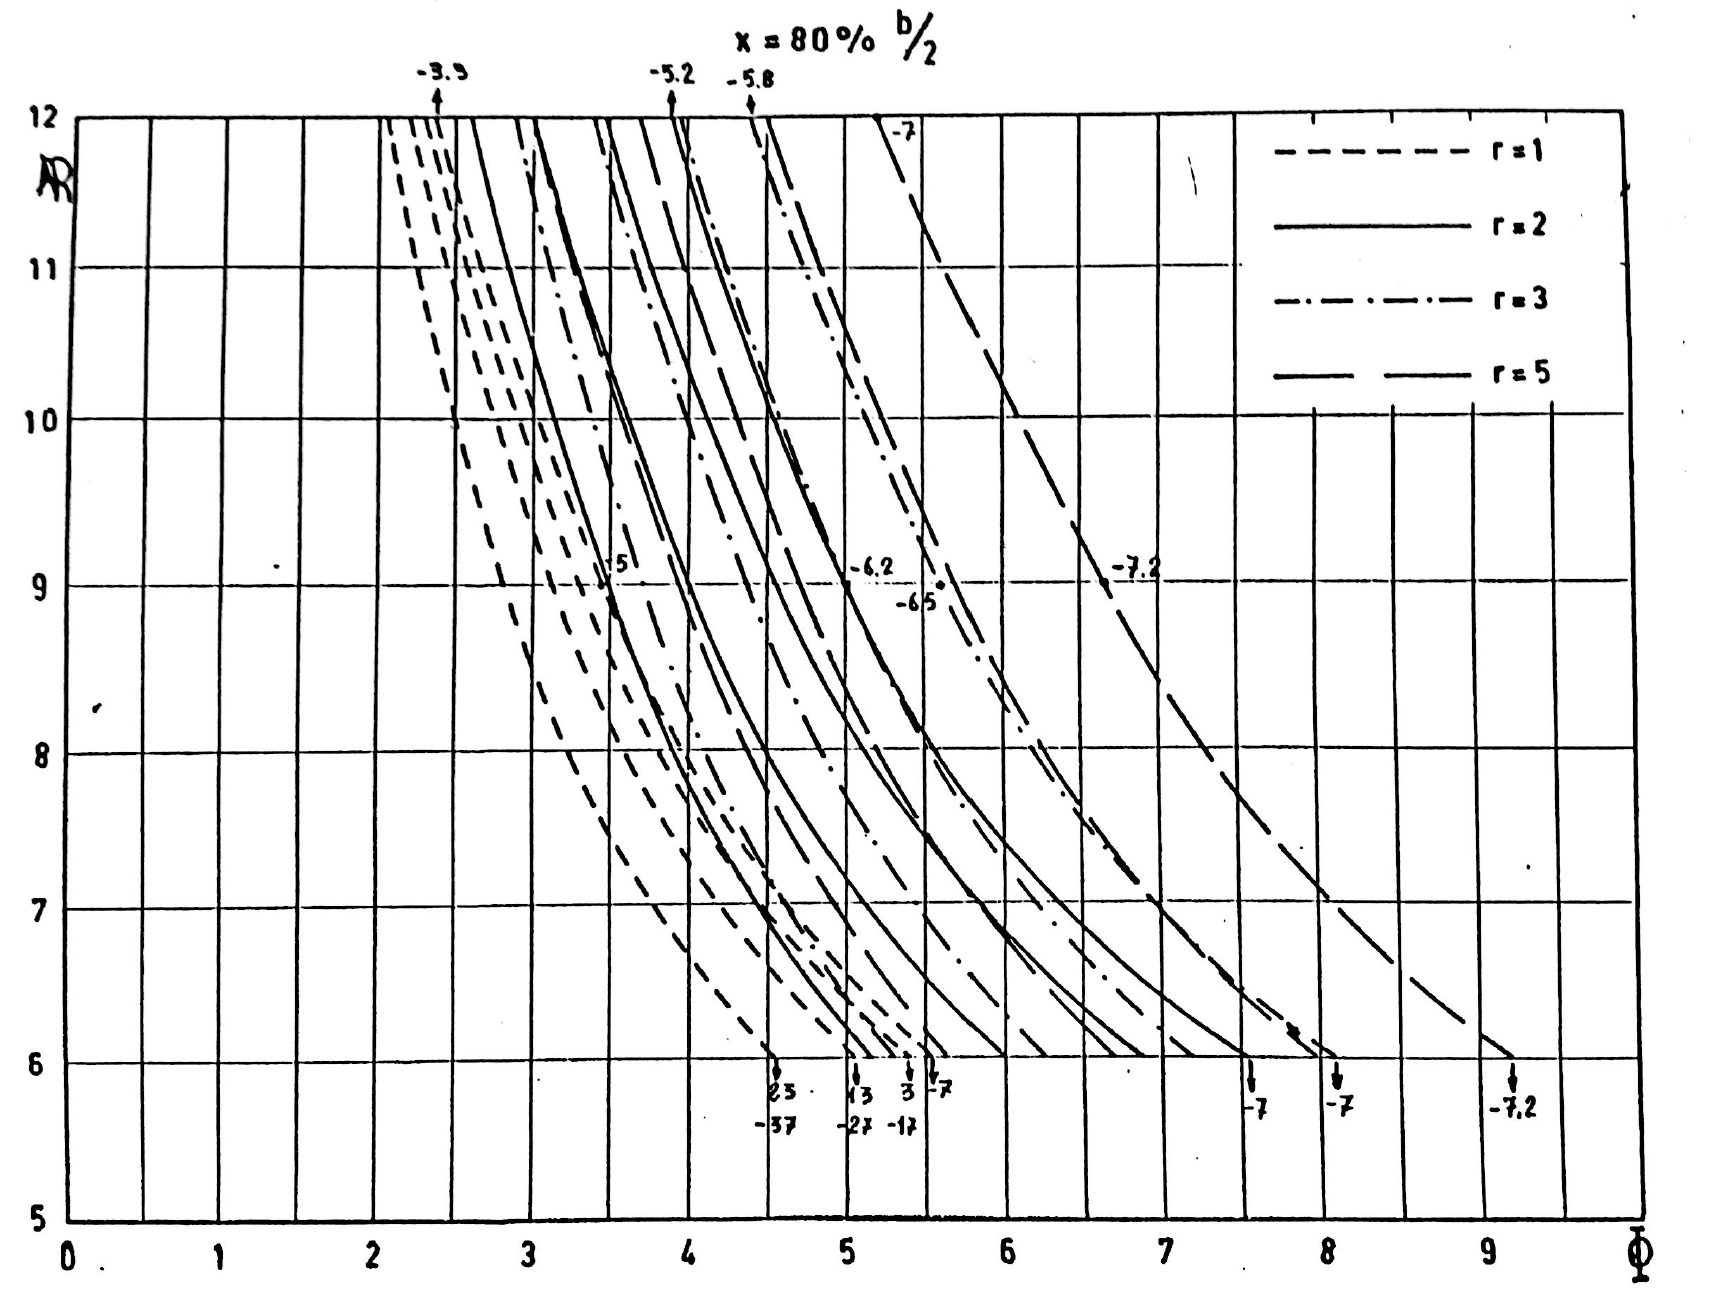
\includegraphics[height=9cm]{immagini/chartGiordano}} 
\caption{Chart for the evaluation of $\Phi$ for $x=80$}
\label{giordanodata}
\end{figure} 

\begin{figure}[H]
\centering
{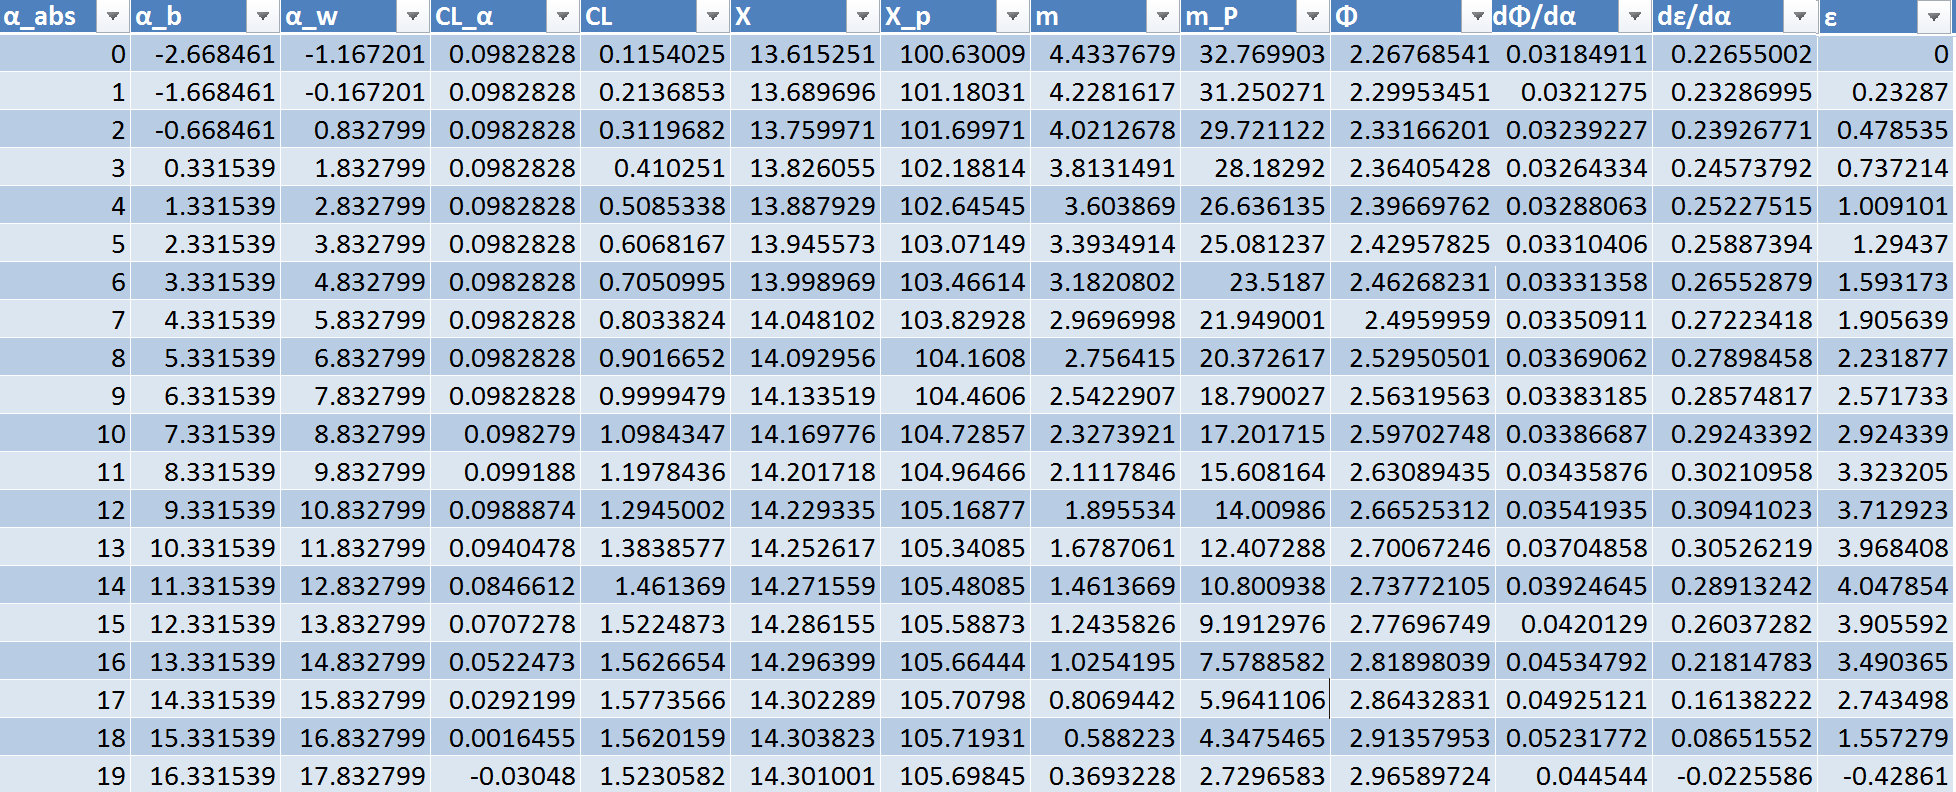
\includegraphics[height=6.6cm]{immagini/giord1.png}} 
\caption{Input and output values of NACA method.}
\label{giordanodata2}
\end{figure} 


\section{Roskam Method}
For the evaluation of downwash ratio at the horizontal tai the following equation at low speed is suggested:

\begin{equation} 
\frac{d\epsilon}{d\alpha} = 4.44 {\left[ K_A K_{\lambda} K_H \sqrt{\cos{ \Gamma_{\frac{c}{4}}}}  \right]}^{1.19}
\end{equation}

Where the K parameters are:

\begin{equation}
K_A = \frac{1}{A} - \frac{1}{1+\AR^{1.7}}
\end{equation}

\begin{equation}
K_{\lambda} = \frac{10 - 3 \lambda}{7}
\end{equation}

\begin{equation}
K_H = \frac{1- \frac{h_H}{b}}{\sqrt[3]{\frac{2 l_H}{b}}}
\end{equation}
\begin{figure}[H]
\centering
{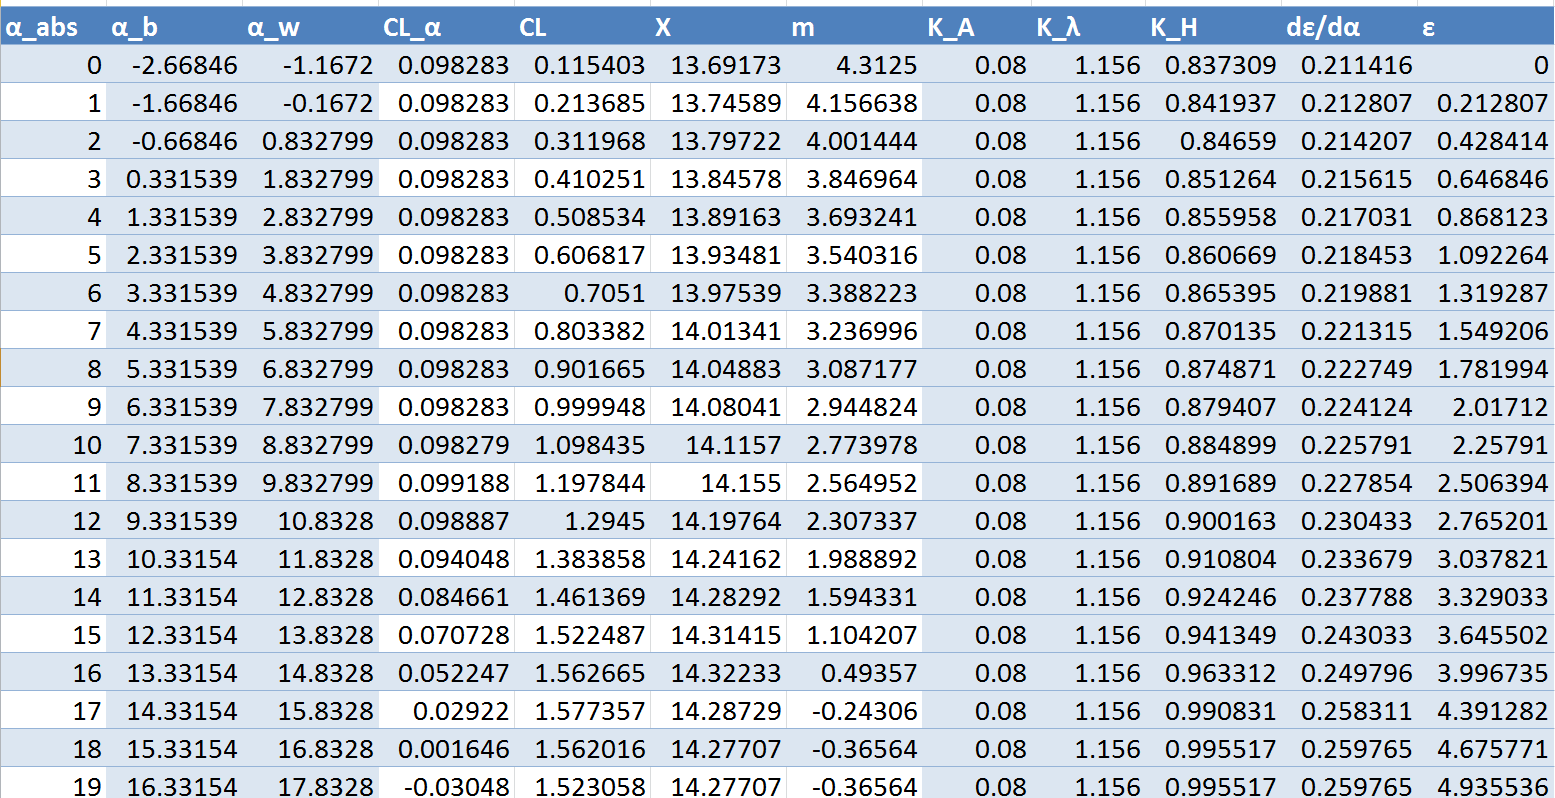
\includegraphics[height=7cm]{immagini/roskam1}} 
\caption{Input and output values of Roskam method.}
\label{roskamdata}
\end{figure} 

This method does not consider a variation of distances with $\alpha$. But the values of $h_H$ and $l_H$ are considered as variable. \\
It's important to notate that in this equation there isn't the $C_{L_{\alpha}}$ contributor so this non linear effect is not considerate. 

\subsection{Results}

As it is possible to see in the following charts the obtained values and the trend are confrontable for low angles of attack. At elevate angles the Roskam method does not see the effect of the reduction of $C_{L_{\alpha}}$.

\begin{figure}[H]
\centering
{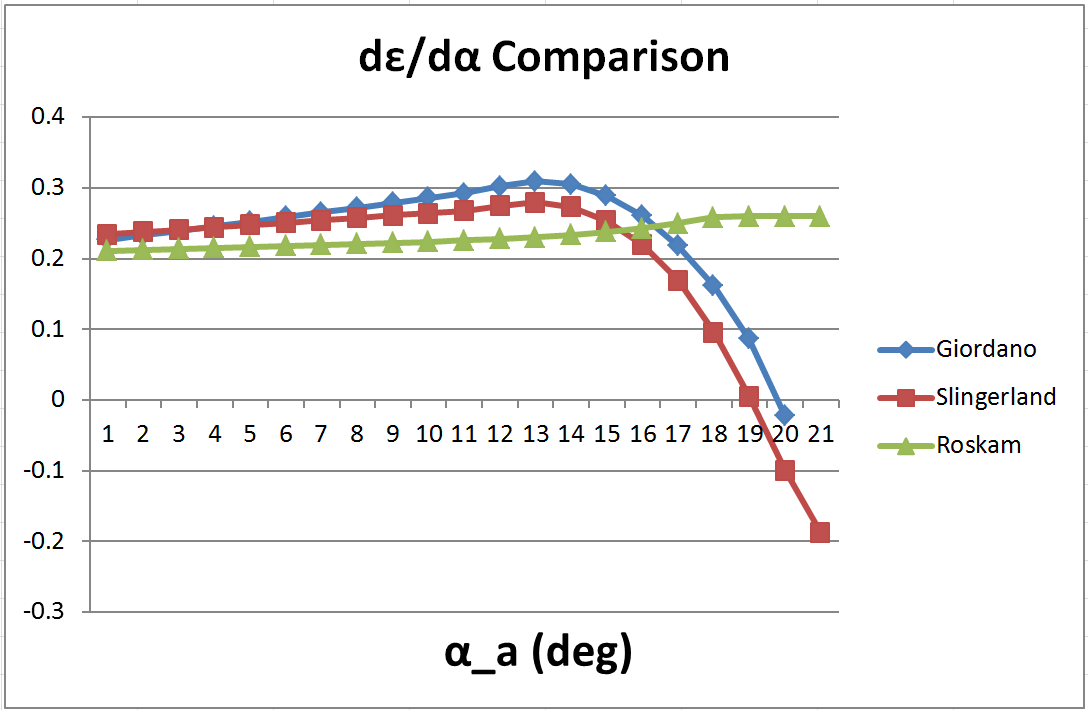
\includegraphics[height=8cm]{immagini/downwashcomparison1}} 
\caption{Results comparison of downwash gradient.}
\label{comparisondownwash}
\end{figure} 

\begin{figure}[H]
\centering
{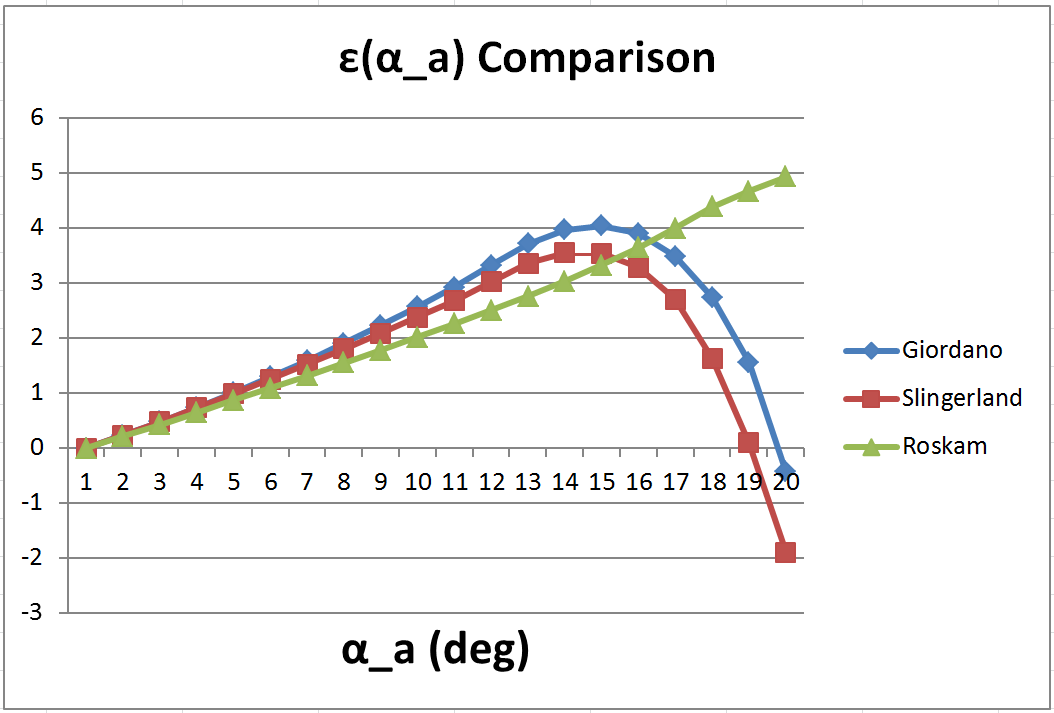
\includegraphics[height=8cm]{immagini/downwashcomparison2}} 
\caption{Results comparison of downwash angle.}
\label{comparisondownwash2}
\end{figure} 

